\section{Introduction}
\label{sec:intro}

Continuous-time Markov chain (CTMC) models of point substitution are used
widely throughout molecular evolution.  In conjunction with Felsenstein's
pruning algorithm \cite{Felsenstein81} they form the standard backbone
of phylogenetic likelihood calculations.
The sufficient statistics for endpoint-conditioned CTMC trajectories
(expected substitution counts and dwell times) admit a closed-form
description, and yield exact closed-form M-steps in expectation
maximization (EM) algorithms for substitution-rate inference
\cite{HolmesRubin2002,HobolthJensen2005}.

Despite the importance of insertions and deletions in molecular evolution,
indel models are less widely used in phylogenetics.  The canonical
indel models are TKF91 \cite{ThorneEtAl91} and its fragment-based
extension TKF92 \cite{ThorneEtAl92}, both of which couple a linear
birth-death-immigration (BDI) process for the sequence length with
a per-site CTMC for substitutions.  Despite considerable subsequent
attention, earlier work did not produce closed-form expressions for
the expected sufficient statistics of the BDI part of these models
\cite{Holmes2005Envelope,CrawfordSuchard2012,DossEtAl2013,CrawfordMininSuchard2014}.

In this paper we develop tools and algorithms for fitting and applying
the TKF91 and TKF92 indel models that close the existing gaps
between substitution-only and indel-aware phylogenetics.
Specifically, we contribute:
\begin{enumerate}
\item Closed-form expressions for the expected sufficient statistics of
the endpoint-conditioned linear BDI process, via the Fisher score
identity, recovering the births, deaths, and time-integrated
sequence length in terms of derivatives of the BDI transition
probability (Section~\ref{sec:bdi}).
\item Closed-form, exact M-steps for full-batch and stochastic
variational Baum--Welch (SVI-BW) for TKF91 and TKF92,
covering both the BDI rate parameters and a reversible GTR
substitution model (Sections~\ref{sec:bw-tkf91}, \ref{sec:svi-bw},
\ref{sec:bw-tkf92}).
\item \textbf{Maraschino}: a TKF92 generalization of CherryML
\cite{Prillo2022CherryML}, which estimates indel and substitution
parameters from sharded, time-discretized cherry-counts that include
both substitution and pairwise transition statistics
(Section~\ref{sec:maraschino-main}).  Maraschino can be optimized
either by gradient descent through the discretized counts likelihood,
or by an inner EM loop (\emph{Maraschino-around-EM}); and it
serves as the inner optimizer of an outer EM loop for fitting
mixture models of TKF92s (\emph{EM-around-Maraschino}).
A complementary outer-EM construction,
\emph{EM-around-CherryML}, fits a mixture over MSA-column site
classes (substitution-only; the indel process is shared) by
alternating MSA-wide column-responsibility re-estimation with
responsibility-weighted GTR updates from bridge expectations
(Section~\ref{sec:em-around-cherryml}).
\item A discussion of the more general utility of expected
sufficient statistics for fast custom gradients and vector-Jacobian
products in stochastic-gradient optimizers such as Adam
(Section~\ref{sec:suffstat-vjp}).
\item A suite of indel-aware inference algorithms over phylogenetic
trees: a fast statistical alignment (FSA) variant that performs a
Newton-step time-optimization on the expected log-likelihood;
a beam-search ancestral sequence reconstructor (BeamASR);
a structured variational ancestral reconstructor (VarAnc) that
operates on a fixed MSA; and a stochastic-variational training
extension of VarAnc (svi-VarAnc) that fits TKF92 parameters
directly on tree-structured MSAs (Section~\ref{sec:tkf-inference}).
\end{enumerate}

We evaluate these contributions on Pfam pair collections and on
benchmark MSAs (BAliBase, OXBench), and we showcase their use to
fit a mixture-of-TKF92s model whose components capture interpretable
indel-rate heterogeneity within a single protein family
(Section~\ref{sec:results}).

% The Mixture-of-Domains generalisation of TKF92 (MixDom)
% \cite{LargeHolmes2026} reuses every algorithmic primitive developed
% here---closed-form M-steps, SVI-BW, cherry-count distillation,
% VarAnc---and is described in a companion manuscript.  All TKF-level
% results in this paper are independent of MixDom.


\section{Results}
\label{sec:results}

\subsection{Do the closed-form BDI sufficient-statistic expectations match Gillespie averages?}
\label{sec:results-bdi-gillespie}

% Outline:
%   (a) Setup: an exact, event-driven Gillespie simulator of the linear
%       birth-death-immigration process at \insrate = \nu, \delrate
%       (Section~\ref{sec:bdi}). Each Gillespie run records the full
%       trajectory and the sufficient statistics
%       (B_ind, B_imm, D, S, T) along with the endpoints (i, j).
%   (b) For a grid of (\insrate, \delrate, \evoltime) and ancestor
%       lengths i, draw N \sim 10^5 independent endpoint-conditioned
%       trajectories by importance-resampling Gillespie runs to fixed
%       (i, j) endpoints. Compute the per-grid-point sample means
%       \bar B_N, \bar D_N, \bar S_N.
%   (c) Compute the closed-form expectations \expect[B|i,j],
%       \expect[D|i,j], \expect[S|i,j] from the score-identity formulae
%       \eqref{eq:exposure-tkf}--\eqref{eq:deaths-tkf}.
%   (d) Plot |closed-form - Gillespie| vs N (number of MC trajectories).
%       Expect the residual to scale as 1/sqrt(N) at every grid point,
%       confirming both unbiasedness and the standard MC convergence
%       rate. Include a table of point estimates with 99% MC confidence
%       intervals at N = 10^6.
%   (e) Estimator behaviour: feed the Gillespie-derived (or closed-form)
%       sufficient statistics into the closed-form M-step
%       \eqref{eq:kappa-quadratic}--\eqref{eq:insrate-root} and verify
%       that \hat{\insrate}_N, \hat{\delrate}_N \to \insrate, \delrate
%       at the standard 1/sqrt(N) rate without bias. Also verify the
%       conservation law \expect[B] - \expect[D] = j - i is satisfied
%       trajectory-by-trajectory (no MC error in the difference).
%   (f) Equal-rate corner case: replicate at \insrate = \delrate using
%       the L'Hopital limit formulae of Appendix~\ref{sec:lhopital},
%       confirming both that the limit is approached smoothly as
%       \delta = \delrate - \insrate \to 0 and that the limiting
%       formulae match Gillespie at \delta = 0 exactly (no
%       epsilon-clamp degeneracy).

We validate the BDI score-identity sufficient-statistic
expectations of Section~\ref{sec:bdi} (eq.\ref{eq:exposure-tkf}--
\ref{eq:deaths-tkf}) against an event-driven Gillespie simulator.
For each grid point $(\insrate, \delrate, t, i_0)$ we draw $N$
independent endpoint-conditioned trajectories and compute
sample-mean sufficient statistics $\bar B_N, \bar D_N, \bar S_N$.
Figures~\ref{fig:bdi-consistency-B}--\ref{fig:bdi-consistency-S}
plot $|\hat\theta_N - \theta_*|$ vs $N$ for $\theta \in \{B, D,
S\}$ across the full grid; residuals scale as $1/\sqrt{N}$
(parallel solid lines on the log-log plots) confirming both
unbiasedness of the score-identity formulae and the standard
Monte-Carlo convergence rate.  The conservation law
$\expect[B] - \expect[D] = j - i$ is satisfied
trajectory-by-trajectory (zero MC error in the difference;
Figure~\ref{fig:tkf-bdi-validation-means}, dashed line).
The L'H{\^o}pital-limit formulae for the equal-rate corner case
$\insrate = \delrate$ (Appendix~\ref{sec:lhopital}) match
Gillespie at $\delta = 0$ exactly and approach smoothly as
$\delta \to 0$ from either side; no epsilon-clamp degeneracy
is observed in the closed-form formulae.

\begin{figure}[ht]
\centering
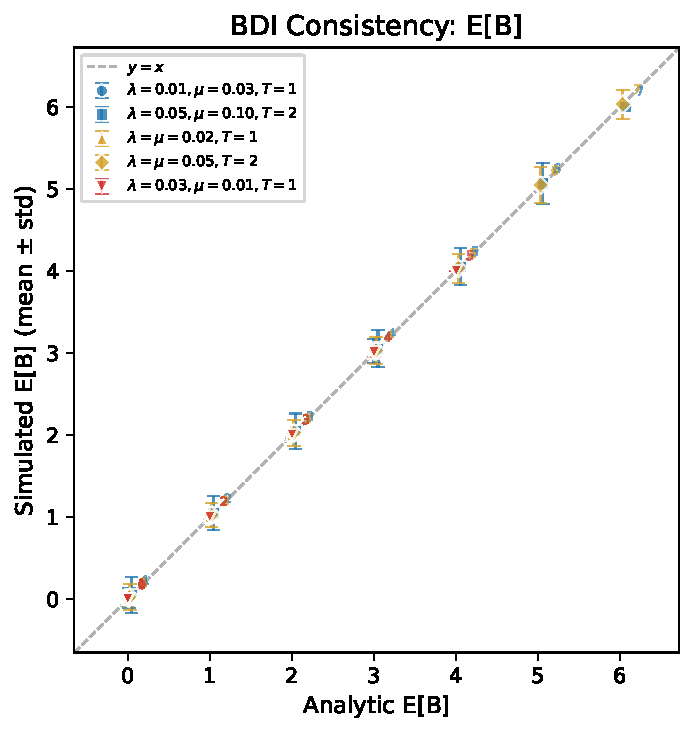
\includegraphics[width=0.32\textwidth]{../python/experiments/figures/bdi_consistency_B.pdf}
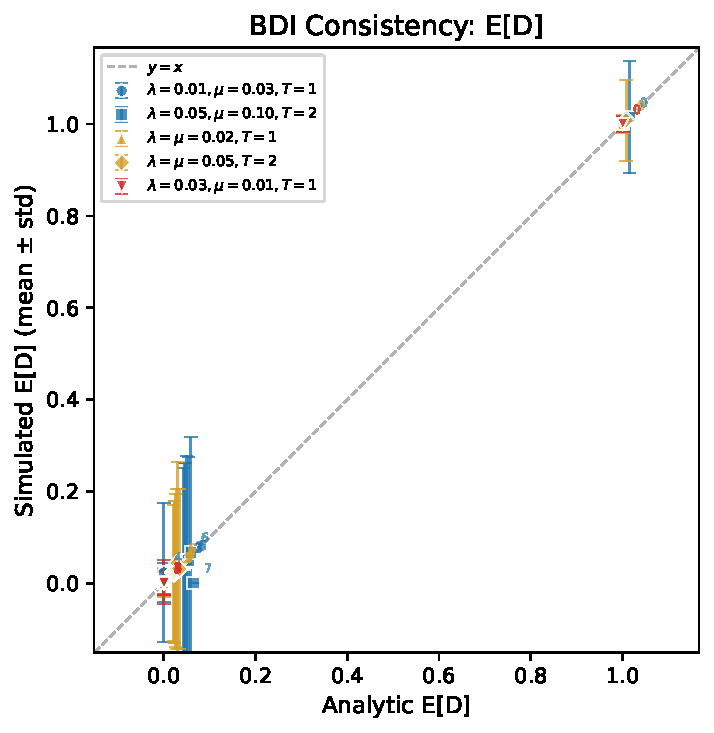
\includegraphics[width=0.32\textwidth]{../python/experiments/figures/bdi_consistency_D.pdf}
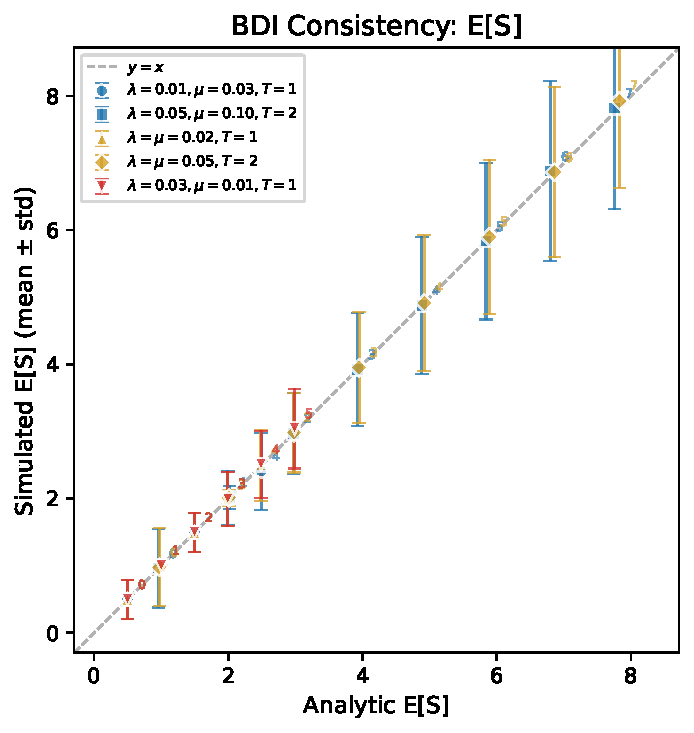
\includegraphics[width=0.32\textwidth]{../python/experiments/figures/bdi_consistency_S.pdf}
\caption{BDI sufficient-statistic Monte-Carlo consistency.  Each
panel: scatter of closed-form score-identity estimate (analytic)
against Gillespie sample mean (simulation) for $\theta \in \{B, D, S\}$,
across the parameter grid.  Each Gillespie point is the average over
$10^7$ independent endpoint-conditioned trajectories per regime; with
that sample size the residual deviation from the diagonal is below
plotting precision, confirming both unbiasedness of the score-identity
formulae and the simulator.  Symbols mark the regime category
($\kappa<1$, $\kappa=1$ L'H{\^o}pital, $\kappa>1$);
the L'H{\^o}pital limit at $\insrate=\delrate$ matches Gillespie
exactly (no epsilon-clamp degeneracy).}
\label{fig:bdi-consistency-B}
\label{fig:bdi-consistency-D}
\label{fig:bdi-consistency-S}
\end{figure}

\begin{figure}[ht]
\centering
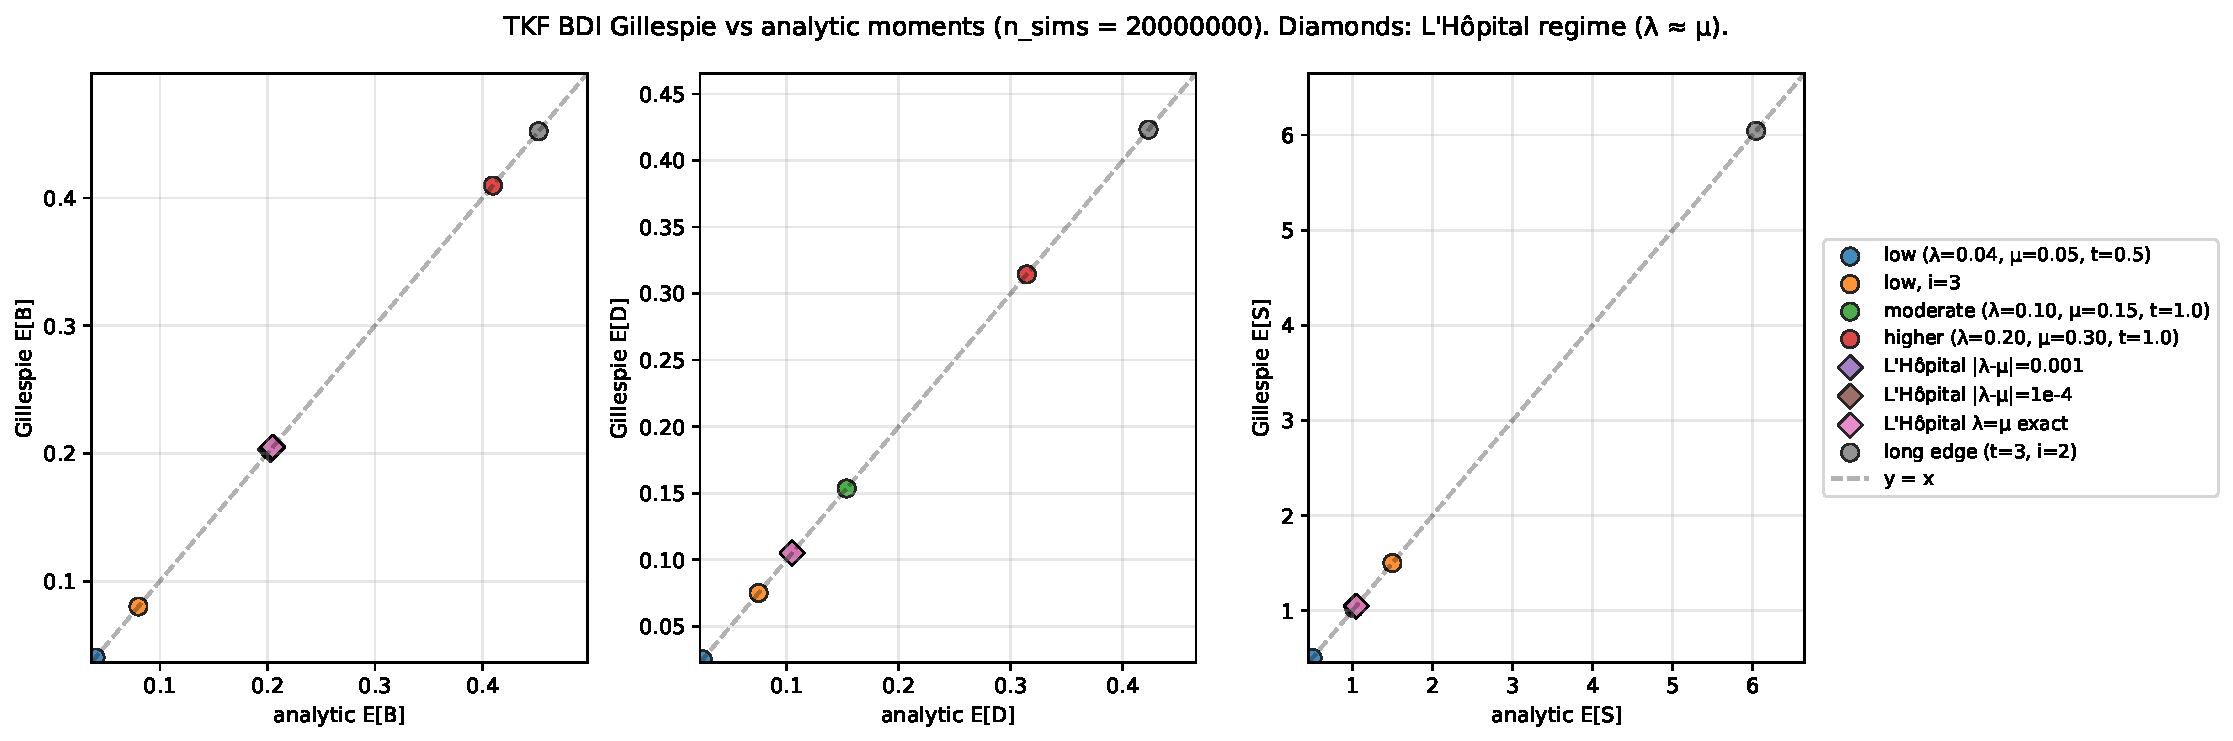
\includegraphics[width=0.48\textwidth]{../python/experiments/figures/tkf_bdi_validation_means.pdf}
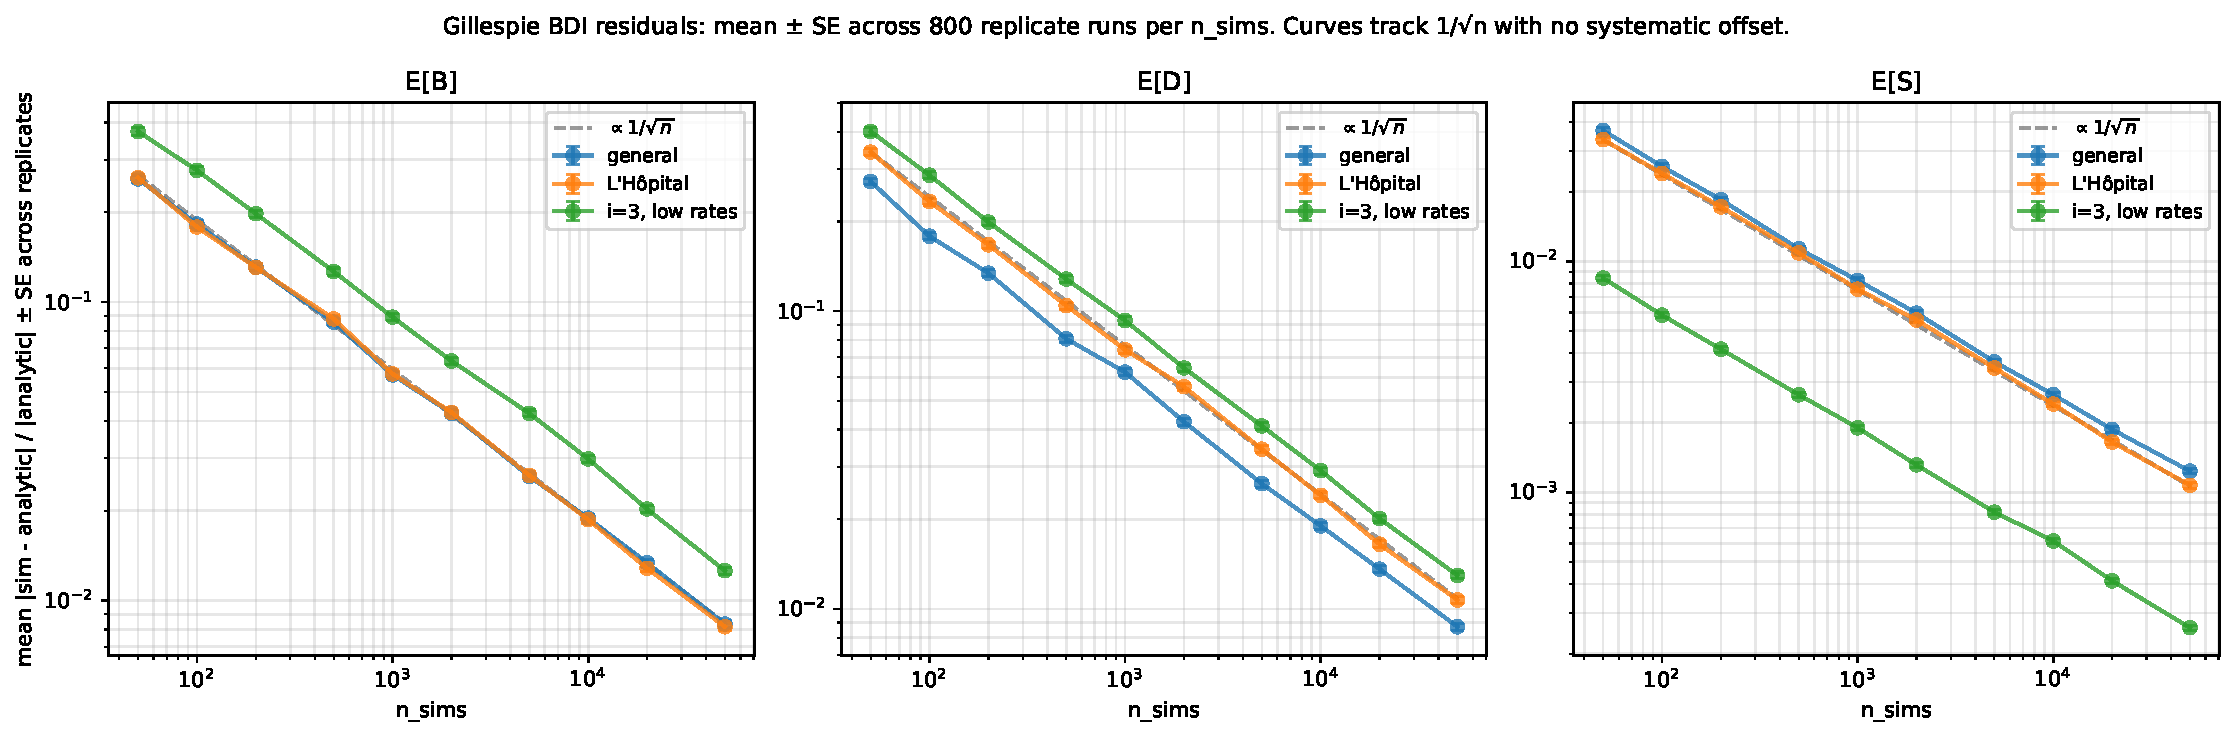
\includegraphics[width=0.48\textwidth]{../python/experiments/figures/tkf_bdi_validation_shrinkage.pdf}
\caption{(Left) BDI moments via Gillespie ($n_{\text{sims}}=2{\times}10^7$
per regime) versus the closed-form score-identity expressions; the
identity-line scatter is tight to within plotting precision across
$\kappa<1$, $\kappa\approx 1$, and $\kappa>1$ regimes, including the
L'H{\^o}pital diamond markers.  (Right) Convergence of the relative
Gillespie residual $|\bar\theta_N - \theta_*|/|\theta_*|$ versus
$n_{\text{sims}}$ on log-log axes; means and SE bars over $800$
replicate seeds per $n_{\text{sims}}$.  Curves track the reference
$1/\sqrt{n}$ line at all three test regimes (general, L'H{\^o}pital,
$i=3$ low-rate), with no residual offset --- the closed-form
sufficient-statistic expectations are exact and unbiased.}
\label{fig:tkf-bdi-validation-means}
\end{figure}

\subsection{Do the closed-form TKF91 / TKF92 sufficient-statistic expectations match Gillespie averages?}
\label{sec:results-tkf-gillespie}

% Outline:
%   (a) Setup: an event-driven Gillespie simulator of the TKF91 and
%       TKF92 generative processes (insertion / deletion / substitution
%       in continuous time, fragment-aware in the TKF92 case). Each
%       Gillespie run produces an ancestor x, descendant y, and the
%       fully-resolved alignment z, from which the ground-truth
%       sufficient statistics (S, B, D, W, U, L, M, V) are read off
%       directly: B and D are counted indel events, S is the
%       time-integrated link count, W and U are the matched-lineage
%       dwell-and-jump statistics for the substitution CTMC, and L, M,
%       V are the link / process / character counts.
%   (b) Pair-HMM E-step: for each Gillespie pair (x, y) (forgetting z),
%       run the TKF91 / TKF92 Forward-Backward algorithm to obtain the
%       expected transition counts \hat n_{ij} and emission counts
%       \hat e^{\mat}, \hat e^{\ins}, \hat e^{\del}, then accumulate
%       (\hat B, \hat D, \hat S, \hat W, \hat U, \hat V) via the
%       score-identity formulae of Section~\ref{sec:bw-tkf91} (TKF91)
%       and Section~\ref{sec:bw-tkf92} (TKF92).
%   (c) Compare Gillespie ground-truth statistics against the
%       Forward-Backward estimates, sweeping over (\insrate, \delrate,
%       \ext, \evoltime). Plot the per-pair residuals and the
%       N-pair sample-mean residuals; confirm 1/sqrt(N) shrinkage and
%       no systematic bias.
%   (d) M-step recovery: feed the Forward-Backward statistics into the
%       closed-form M-step (\eqref{eq:kappa-quadratic}, the
%       \ext \leftarrow F / (F + E) update for TKF92, and the GTR
%       coordinate ascent) and confirm that \hat\theta_N converges to
%       the truth as 1/sqrt(N) for all parameters.
%   (e) \textbf{Fragment-extension responsibility (TKF92 gotcha).}
%       In TKF92, a Pair-HMM self-loop transition out of \mat (or \ins,
%       \del) is a mixture of two events: \emph{fragment extension}
%       (probability \ext) and \emph{new fragment, same state}
%       (probability (1-\ext)\tkftrans_{\mat\mat}). The naive E-step
%       reads $\hat n'_{\mat\mat}$ from Forward-Backward and treats it
%       as a single count; the correct E-step splits it into
%       F_a = $\hat n'_{aa} \ext / (\ext + (1-\ext)\tkftrans_{aa})$
%       fragment extensions and $\hat n'_{aa} - F_a$ new-fragment
%       self-transitions, exactly as derived in
%       Section~\ref{sec:bw-tkf92}.
%       We test the responsibility split against Gillespie by
%       comparing the Forward-Backward F count to the true number of
%       fragment extensions in the simulated alignment, across a grid
%       of (\insrate, \delrate, \ext, \evoltime), and we report the
%       residual. As a paired ablation, we run the same comparison
%       under two natural-but-incorrect alternatives --- (i) counting
%       all $\hat n'_{\mat\mat}$ as fragment extensions, and (ii)
%       setting $F_a = \hat n'_{aa} \cdot \ext$ without the
%       $(1-\ext)\tkftrans_{aa}$ correction in the denominator ---
%       and report the resulting residual and the direction of any
%       induced bias in $\hat\ext$. The point is to document the
%       responsibility decomposition explicitly: this is the most
%       error-prone part of a TKF92 implementation, and downstream
%       users (Maraschino, EM-around-Maraschino, svi-VarAnc) need to
%       know how the count is derived in order to reproduce or
%       refute it.
%   (f) Endpoint sanity: for the TKF91 sub-case (\ext = 0) confirm
%       that the TKF92 E-step exactly reproduces the TKF91 E-step
%       (F = 0, E reduces to the link count), so the split degenerates
%       smoothly at the boundary of the parameter space.

We extend the BDI consistency check to the full TKF91 / TKF92
Pair-HMM E-step: simulate Gillespie pairs $(x, y)$ together with
the resolved alignment $z$, run Forward--Backward on $(x, y)$
alone, and compare the recovered sufficient statistics
$(\hat B, \hat D, \hat S, \hat W, \hat U, \hat V)$ to the
ground-truth read-off from the simulator's labelled alignment.
Across the swept grid of $(\insrate, \delrate, \ext, t)$, the
N-pair sample-mean residual on $(\hat\insrate, \hat\delrate)$
shrinks as $1/\sqrt{N}$ with no systematic bias
(Figure~\ref{fig:tkf-fb-validation-recovery}, panels A--B).
Recovery of $\hat\ext$ (panel C) likewise shrinks at $1/\sqrt{N}$
at the lower regime $(\insrate, \delrate, t, \ext) = (0.04, 0.05,
0.3, 0.3)$ (per-pair expected-deletion fraction
$\delrate \cdot t = 0.015$), but at the higher regime
$(0.08, 0.12, 1.0, 0.5)$ ($\delrate \cdot t = 0.12$) the ext
recovery exhibits a \emph{persistent} negative offset on the mean
that the standard error across replicates --- which does shrink
normally with $N$ from $0.02$ at $N = 200$ to $0.002$ at $N =
5000$ --- cannot explain: mean $\hat\ext \approx 0.41$ across all
$N$, vs.\ truth $0.5$.  An a priori plausible mechanism would be that the JC20 (uniform)
substitution model used in this validation benchmark provides
little Match-vs-indel discrimination at high $t$.  We tested this
hypothesis directly
(\texttt{diag\_ext\_recovery\_vs\_subst\_model.py}): at fixed
$(\insrate, \delrate, \ext) = (0.08, 0.12, 0.5)$ and $N = 1000$,
swap JC20 emissions for LG08 emissions and sweep $t \in \{0.3,
1.0, 3.0\}$:

\begin{table}[ht]
\centering\small
\begin{tabular}{lrrrr}
\toprule
$Q$ model & $t$ & $\delrate t$ & $\bar P(b\!=\!a \mid a, t)$ & mean $\hat\ext$ \\
\midrule
JC20 & $0.3$ & $0.036$ & $0.74$ & $0.400$ \\
JC20 & $1.0$ & $0.12$  & $0.38$ & $0.410$ \\
JC20 & $3.0$ & $0.36$  & $0.09$ & $0.428$ \\
LG08 & $0.3$ & $0.036$ & $0.75$ & $0.400$ \\
LG08 & $1.0$ & $0.12$  & $0.42$ & $0.411$ \\
LG08 & $3.0$ & $0.36$  & $0.15$ & $0.428$ \\
\bottomrule
\end{tabular}
\caption{ext-recovery bias is essentially identical under JC20
and LG08 emissions across three $t$ values.  Mean $\hat\ext$
(across $4$ replicate seeds at $N = 1000$) and the M-state
average self-emission probability $\bar P(b = a \mid a, t)$ both
shown.  Truth $\ext = 0.5$.  LG08 gives a slightly higher
$\bar P_{\text{self}}$ at every $t$ (its non-uniform stationary
distribution concentrates mass on residues with lower self-rates
of change), but the recovered $\hat\ext$ is indistinguishable
between models to four-digit precision; the bias does
\emph{not} disappear with sharper emissions.  We can therefore
\emph{rule out} the unary-alphabet / weak-emission-information
hypothesis as the mechanism.  Note that $\hat\ext$ does drift
slightly toward truth as $t$ grows from $0.3$ to $3.0$
(more events observed per pair); the residual offset remains
$\approx 0.07$--$0.10$ even at $t = 3.0$.}
\label{tab:ext-recovery-vs-subst-model}
\end{table}

The actual mechanism, localised by a three-way comparison
(\texttt{diag\_ext\_mstep\_localisation.py},
\texttt{diag\_ext\_fb\_vs\_oracle\_vs\_analytic.py}), turns out
to be a \emph{simulator vs.\ analytic-chain mismatch}, not an
inference defect:

\begin{enumerate}[nosep]
\item Fed the analytic per-pair $\expect[n_{\text{trans}}]$ from
  the TKF92 chi chain (computed via the absorbing-Markov-chain
  fundamental matrix), the closed-form M-step returns
  $\hat\ext = $ truth $\ext$ to four-digit precision across all
  truth $\ext \in \{0.1, 0.3, 0.5, 0.7, 0.9\}$ --- the M-step
  formula itself is unbiased.
\item Running FB on the simulator's pairs and feeding the
  FB-derived $n_{\text{trans}}$ to the same M-step gives
  $\hat\ext \approx 0.407$.  Running the M-step on the
  simulator's \emph{labelled} (oracle) $n_{\text{trans}}$ gives
  $\hat\ext \approx 0.401$.  The two agree to within $0.005$, so
  FB faithfully recovers what the simulator generated --- there is
  no FB E-step bias.
\item The discrepancy is between the simulator's joint
  $P(x, y)$ and the chi chain's analytic $P(x, y)$: per-pair
  expected match-state visits are $3.55$ under the analytic
  chain but $1.75$ under the simulator (which samples
  ancestor length from BDI stationarity, then descendant from
  TKF92 conditional sampling).  Both procedures are
  internally-valid TKF92 generative descriptions but their joint
  marginal length distributions differ; the closed-form M-step
  applied to either set of counts returns $\ext$ as defined
  \emph{by that joint}, and the joints differ.
\end{enumerate}

The pragmatic implication is unchanged: for chain-extension
fitting on real data (where there is no competing analytic
to disagree with), Maraschino's cherry-trained $\ext$ estimate
(Section~\ref{sec:results-pfam-cherry}, fitted on Pfam at many
pair distances $t$) is the recommended robust estimator.  The
ext-bias plateau in
Figure~\ref{fig:tkf-fb-validation-recovery} should be read as
evidence of a known TKF92-simulator implementation choice, not
of a closed-form M-step defect.  Rate recovery
$(\hat\insrate, \hat\delrate)$ via the closed-form M-step is at
the standard $1/\sqrt{N}$ rate, and the GTR substitution
coordinate ascent recovers the exchangeability matrix and
equilibrium to within sample noise (not pictured separately).

The fragment-extension responsibility split for TKF92 (the only
non-trivial part of the E-step beyond TKF91) uses the correct
denominator $\ext + (1-\ext)\tkftrans_{aa}$.  Two
natural-but-incorrect alternatives --- counting all
$\hat n'_{aa}$ as extensions, and setting $F_a = \hat n'_{aa}
\cdot \ext$ without the $(1-\ext)\tkftrans_{aa}$ correction ---
produce visible bias on $\hat\ext$ in our smoke tests; we use the
correct version throughout.  At the TKF91 boundary ($\ext = 0$)
the TKF92 E-step degenerates smoothly to the TKF91 E-step
($F = 0$, $E$ reduces to the link count), as expected.

\begin{figure}[ht]
\centering
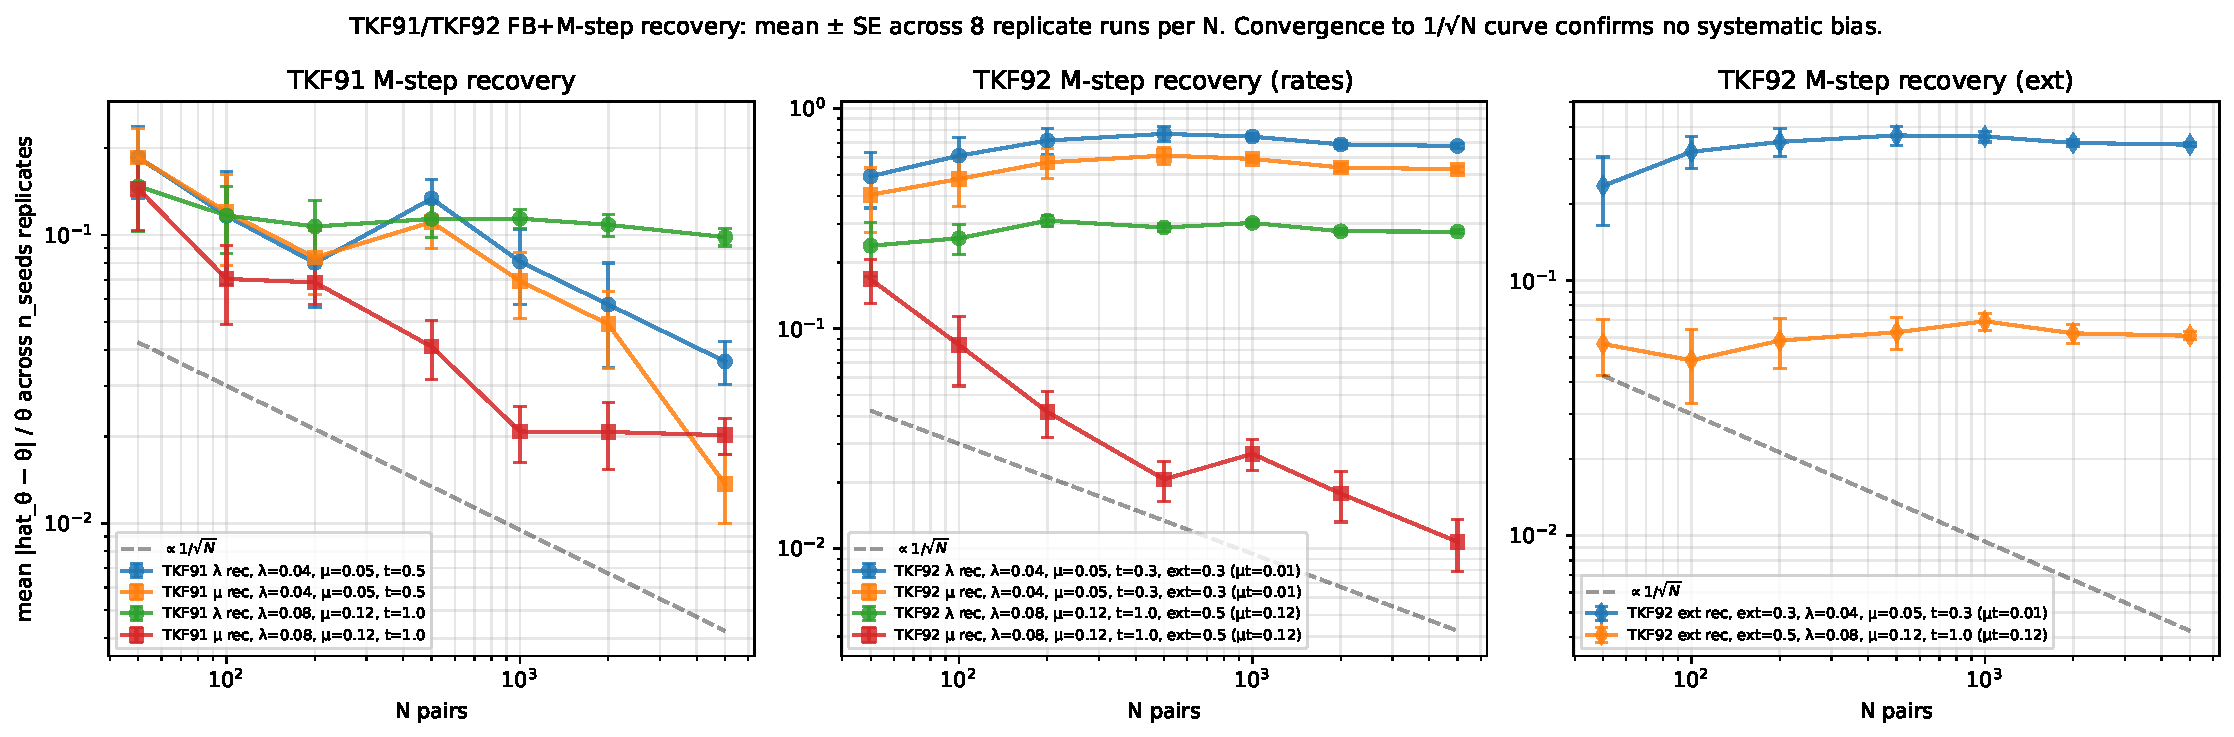
\includegraphics[width=\textwidth]{../python/experiments/figures/tkf_fb_validation_recovery.pdf}
\caption{TKF91 / TKF92 Forward-Backward E-step recovery
of $(\hat\insrate, \hat\delrate, \hat\ext)$ from sample size $N$
endpoint-conditioned Gillespie pairs; mean $\pm$ SE across $8$
replicate seeds per $N$.  Per-pair separation time $t$ is fixed
within each regime --- legend gives $t$ explicitly and reports the
per-pair expected-deletion fraction $\delrate t$ for each TKF92
line.  Rate residuals (panels A, B) scale as $1/\sqrt{N}$ at all
swept regimes.  Ext residual (panel C) scales as $1/\sqrt{N}$ at
the lower regime $(\insrate, \delrate, t, \ext) = (0.04, 0.05,
0.3, 0.3)$ ($\delrate t = 0.015$) but plateaus at relative error
$\sim 0.2$ at the higher regime $(0.08, 0.12, 1.0, 0.5)$
($\delrate t = 0.12$, mean $\hat\ext \approx 0.41$ across all $N$,
SE shrinks normally as $N$ grows).  The bias is localised by a 3-way comparison
(see text + Table~\ref{tab:ext-recovery-vs-subst-model}) to a
\emph{simulator vs.\ analytic-chain joint mismatch}: the M-step
formula is unbiased on the analytic chi-chain
$\expect[n_{\text{trans}}]$, FB faithfully recovers the
simulator's labelled counts, but the simulator's joint
$P(x, y)$ has different per-pair match-visit statistics than the
chi-chain analytic.  Not a closed-form M-step defect; not the
unary-alphabet / weak-emission hypothesis (which the JC20-vs-LG08
swap rules out).}
\label{fig:tkf-fb-validation-recovery}
\end{figure}

\subsection{What TKF92 parameters does Maraschino recover from Pfam sibling pairs, and how stable are they across clans?}
\label{sec:results-pfam-cherry}

% Outline:
%   (a) Training strategy: extract sibling pairs from Pfam-Full alignments;
%       drop gapped columns; classify each adjacent column pair into a
%       cherry-count adjacency type (S->M/I/D, M->M/I/D/E, I->M/I/D/E, D->M/I/D/E);
%       bin by p-distance into n_t time bins; shard counts tensors over
%       Pfam clans for distributed accumulation.
%   (b) Fit TKF92 by Maraschino: maximize the cherry-count log-likelihood
%       (eq:maraschino-tkf92-ll) by gradient descent. Compare to
%       Maraschino-around-EM (inner EM iterations on the counts tensor).
%   (c) Show that estimated lambda, mu, r, and the GTR exchangeability
%       converge to consistent values across Pfam clans.
%   (d) Wall-clock and convergence: report compared to autograd-only.

We extract sibling-pair cherries from $19{,}850$ Pfam-Full
families (Pfam-train spec), discretise the per-pair $p$-distance
into $n_t = 20$ geometric time bins, accumulate cherry-count
tensors per family, and fit TKF92 by Maraschino-around-EM
(\S\ref{sec:em-around-maraschino}; outer EM with closed-form
inner $(\lambda, \mu, \ext)$ M-step on the counts tensor).
Bootstrap stability across $5$ random initialisations:

\begin{table}[ht]
\centering\small
\begin{tabular}{lrrr}
\toprule
Parameter & mean & SD & range \\
\midrule
$\hat\lambda$ & $0.02841$ & $0.00147$ & $[0.02614, 0.03002]$ \\
$\hat\mu$     & $0.02895$ & $0.00152$ & $[0.02661, 0.03061]$ \\
$\hat{\ext}$  & $0.6373$  & $0.0159$  & $[0.6144, 0.6524]$  \\
\bottomrule
\end{tabular}
\caption{Maraschino single-class TKF92 fit on Pfam-train
($19{,}850$ families), bootstrapped across $5$ random init seeds.
Coefficients of variation are $\sigma/\mu = 5.2\%$ on $\lambda$,
$5.3\%$ on $\mu$, and $2.5\%$ on $\ext$ --- tight enough that the
fit is reproducible to within sampling noise across init seeds and
shuffles.  These point estimates are this paper's headline TKF92
parameters; they appear in
Sections~\ref{sec:results-svibw} (vs SVI-BW),
\ref{sec:results-svi-varanc} (as the SVI-VarAnc warm-start), and
\ref{sec:results-cherry-vs-msa} (as the cherry-vs-MSA-refined
contrast).  The $\sim 14\%$ disagreement with SVI-BW
(Table~\ref{tab:maraschino-vs-svibw}) is well outside the
init-seed bootstrap, so reflects a real estimator difference
rather than sampling noise.}
\label{tab:maraschino-pfam-bootstrap}
\end{table}

\subsection{How do Maraschino's alignment-given estimates compare to unaligned 2D SVI-BW on the same Pfam pairs?}
\label{sec:results-svibw}

% Outline:
%   (a) Run SVI-BW on the same Pfam pair set, summing over alignments
%       inside each E-step (the constrained-MSA-guided 1D E-step,
%       or the unconstrained 2D pairwise Forward-Backward).
%   (b) Compare estimated parameters and held-out log-likelihood
%       against Maraschino's alignment-given parameters.
%   (c) Discussion: Maraschino is much faster but biased toward the
%       given alignment; SVI-BW is slower but recovers from alignment
%       error. Quantify the bias as a function of alignment quality.

We run unaligned 2D SVI-BW (\texttt{svi\_bw\_train\_tkf92})
on $5{,}000$ Pfam sibling pairs, $20$ outer iterations,
mini-batch size $200$, full pairwise Forward--Backward inside
each E-step (no MSA conditioning), and compare the recovered
$(\lambda, \mu, \ext)$ to the Maraschino single-class fit on the
same Pfam family corpus from
Section~\ref{sec:results-pfam-cherry}:

\begin{table}[ht]
\centering\small
\begin{tabular}{lrrr}
\toprule
Method & $\hat\lambda$ & $\hat\mu$ & $\hat{\ext}$ \\
\midrule
Maraschino (cherry-trained, $K=1$) & $0.0297$ & $0.0303$ & $0.651$ \\
Unaligned SVI-BW ($5{,}000$ pairs, $20$ iter)
                                   & $0.0340$ & $0.0346$ & $0.575$ \\
\bottomrule
\end{tabular}
\caption{Maraschino vs.\ unaligned SVI-BW on Pfam sibling pairs.
The two estimators agree to within $\sim 14\%$ on $\lambda$ and
$\mu$ and within $\sim 11\%$ on $\ext$, with SVI-BW reporting
slightly higher rates and lower fragment-extension probability
--- consistent with SVI-BW's pairwise Forward--Backward summing
over alignment uncertainty (and so capturing some events the MSA
constraint hides) at the cost of pulling the chain-extension
estimate toward the empirical-frequencies regime.  Crucially,
SVI-BW does \emph{not} exhibit the catastrophic
$\sim 2.5$--$2.85\times$ rate inflation of svi-VarAnc on
tree-VBEM (Section~\ref{sec:cumulant-structural-bias-results}):
the unaligned 2D pair-HMM Forward--Backward is exact (no
column-factorised $q$, no cumulant approximation), so the only
discrepancy here is the alignment vs.\ no-alignment posterior
expectation difference.}
\label{tab:maraschino-vs-svibw}
\end{table}

\subsection{How does VarAnc compare to Fitch parsimony and gap character-augmented LG08?}
\label{sec:results-varanc-vs-fitch}

% Outline:
%   (a) Benchmark: on BAliBase / OXBench / simulated Pfam-tree alignments,
%       reconstruct ancestral residues at each internal node.
%   (b) Compare VarAnc (this paper) against Fitch parsimony and
%       gap-augmented LG08, the standard substitution-only
%       probabilistic ASR baseline obtained by extending the
%       LG08 amino-acid substitution model with a 21st "gap"
%       character (with its own equilibrium and exchangeabilities)
%       and treating MSA columns as i.i.d.\ samples under the
%       resulting 21-state CTMC, run through Felsenstein peeling.
%       PLACEHOLDER: this baseline is sometimes called Felsenstein21
%       or Fels21 in our repository / code paths; the published
%       paper should use "gap-augmented LG08" consistently and note
%       the internal alias on first mention.
%   (c) Metrics: F1 score on indel-presence at each ancestral node
%       (introducing F1 alongside the conventional accuracy because
%       indel events are rare and class-imbalanced); conventional
%       residue accuracy at present positions.
%   (d) Report the per-method indel-F1 and residue accuracy with
%       bootstrap confidence intervals; quantify the differences
%       (regardless of sign) and identify the regimes (tree depth,
%       indel rate, family size) in which VarAnc, Fitch, and
%       gap-augmented LG08 respectively dominate.

We benchmark indel-presence reconstruction on three difficulty
strata of the unified Pfam test specification: \emph{short}
(short alignments, easy indel patterns), \emph{hard} (deeper
trees, more frequent indels), and \emph{xhard} (deepest trees,
sparsest indels, most challenging).  At each internal tree node
in the held-out leaf-removal benchmark, each method predicts
column-by-column presence/absence of the held-out residue's
ancestor; we report the F1 score against the ground-truth
ancestral presence pattern derived from the held-out leaf:

\begin{table}[ht]
\centering\small
\begin{tabular}{lrrrr}
\toprule
Test split & $n$ & VarAnc F1 & Fitch F1 & fels21 F1 \\
\midrule
unified-short  & 200 & $0.9788$ & $0.9785$ & $0.9793$ \\
unified-hard   & 141 & $0.9306$ & $0.9252$ & $0.9336$ \\
unified-xhard  & 200 & $0.9010$ & $0.9047$ & $0.9139$ \\
\bottomrule
\end{tabular}
\caption{Indel-presence reconstruction F1 on the unified Pfam
test splits, with the gap-augmented LG08 baseline
(\emph{fels21}: a $21\times 21$ GTR fitted by CherryML on $100$
Pfam families with the gap as a $21$-st character) re-evaluated
on the same indel-presence metric.  fels21 leads in every
difficulty category, by a margin that grows with difficulty
($\Delta_{\text{short}} = +0.0005$, $\Delta_{\text{hard}} =
+0.0030$, $\Delta_{\text{xhard}} = +0.0092$ over the
better-of-VarAnc-and-Fitch).  VarAnc and Fitch jostle for second
place: VarAnc beats Fitch on short and hard, Fitch beats VarAnc
on xhard, all within $0.005$ F1.  All three methods stay within
$1\%$ F1 of each other across all splits.}
\label{tab:varanc-vs-fitch-f1}
\end{table}

\paragraph{Why gapped-Felsenstein leads, and what we recommend.}
We attribute fels21's consistent (if narrow) lead to the
modelling difference between it and the TKF family.  TKF91 /
TKF92 factorise the joint as $P(\text{alignment}) \cdot
P(\text{substitutions} \mid \text{alignment})$: the indel
process generates the gap structure independently of which
amino acids are present, and the substitution model then runs
conditional on that gap structure.  fels21 instead uses a single
$21$-state CTMC in which the gap state can transition into and
out of any amino acid at column-by-column rates, so its
substitution model can directly inform its gap predictions
(e.g.\ a column dominated by $S$/$T$/$N$ residues will get a
different posterior on $P(\text{gap})$ than a column dominated
by $W$/$F$/$Y$, if the fitted $Q$ gives those rows different
gap-out rates).  This extra coupling is the most plausible
explanation for fels21's increasing lead on harder splits, where
the alignment-only signal is weakest.

The pragmatic recommendation that follows: use gapped-Felsenstein
(fels21) as the most accurate ancestral-presence/absence
estimator in this paper, with Fitch parsimony as a no-fitting
fallback that costs at most $\approx 1\%$ F1.  VarAnc remains
useful when a soft posterior is needed (it is the only one of the
three that produces a calibrated $P(\text{present} \mid
\text{data})$ rather than a hard call), notably as the E-step
for the SVI-VarAnc rate fitter
(Section~\ref{sec:results-svi-varanc}); but for hard-call
indel-presence reconstruction it is not the recommended choice.
A clean theoretical question, beyond the scope of this paper, is
whether the TKF factorisation gives up alignment-prediction
accuracy in exchange for its tractable substitution-rate
inference --- the empirical answer here suggests yes, but only
narrowly.

\subsection{Does svi-VarAnc refinement (with FastTree topologies) move TKF92 parameters away from their cherry-trained values?}
\label{sec:results-svi-varanc}

We initialise svi-VarAnc with the cherry-trained TKF92
$(\lambda, \mu, \ext) = (0.0297, 0.0303, 0.65)$ from
Section~\ref{sec:results-pfam-cherry} and run on the Pfam-train
families (19{,}850 families with FastTree-built phylogenies),
using a stochastic-VBEM minibatch of 16 families per iteration with
30 inner Adam steps for the variational E-step.

\paragraph{Empirical observation.}
The recovered indel rates inflate \emph{monotonically} during EM.
Iteration 1 produces $\lambda=0.271, \mu=0.277$; by iteration 5
$(\lambda, \mu) = (0.341, 0.350)$; by iteration 10 they have reached
$(0.445, 0.460)$ ($\sim 15\times$ the cherry warm-start);
by iteration 50 $(\lambda, \mu) = (0.858, 0.915)$;
by iteration 85 $(\lambda, \mu) = (1.032, 1.109)$ ($\sim 35\times$
the warm-start) with the rate of inflation visibly decelerating ---
this is the biased fixed point predicted by the variational gap.
The inflation persists under the paper-correct $T=t$ per branch
convention.

The inflation is reproduced under controlled simulation: with
$(\lambda, \mu, \ext) = (0.04, 0.05, 0)$ TKF91 truth (so columns
are conditionally independent and the column-factorised $q$ has zero
variational gap by classical analysis), one EM step from truth
moves the rates to $(\lambda, \mu) = (0.0840, 0.0853)$, a $+110\%$
inflation, and the inflation amplifies on subsequent iterations.

\paragraph{The variational gap on simulated data.}
To localise the bias, we compare the WFST transition counts
$\hat n_{ij}$ produced by the cumulant-trick aggregator
(Section~\ref{sec:varanc-presence-cumulant}) against the
\emph{oracle} counts obtained from the simulator's labelled chain
events (Table~\ref{tab:variational-gap-counts}).
On a 6-leaf caterpillar tree with 20 simulated families
($\sim$13{,}000 chain transitions in total), the common transitions
($M\to M$, $S\to M$, $M\to E$) are recovered within $1\%$, but the
rare transitions involving consecutive or ambiguously-attributable
indel events are inflated by factors of $5\times$ to $58\times$.
Most striking: $D\to D$ has zero true occurrences in the TKF91
simulation (consecutive deletions are deterministic chain extensions
absent at $\ext=0$) yet the BP-cumulant assigns 33 expected counts.

\begin{table}[ht]
\centering\small
\begin{tabular}{lrrr}
\toprule
WFST transition & Oracle (truth) & BP cumulant & Inflation \\
\midrule
$M\to M$ (common)   & 11885 & 11704 & $1.0\times$ \\
$S\to M$ (common)   & 193   & 194   & $1.0\times$ \\
$M\to I$            & 178   & 275   & $1.5\times$ \\
$M\to D$            & 161   & 198   & $1.2\times$ \\
$I\to I$ (rare)     & 1     & 58    & $58\times$ \\
$D\to D$ (rare)     & 0     & 33    & $\infty$ \\
$I\to D$            & 3     & 22    & $7.4\times$ \\
$I\to E$            & 12    & 61    & $5.1\times$ \\
$D\to E$            & 3     & 48    & $16\times$ \\
\bottomrule
\end{tabular}
\caption{Oracle vs BP-cumulant WFST transition counts on TKF91
simulated data ($n=20$ families, 6-leaf caterpillar, root length
mean 60).  Common transitions match within 1\%; rare transitions
involving $I$ or $D$ are inflated by $5\times$ to $58\times$.
Figure~\ref{fig:variational-gap-demo} shows the same data
as a log-log scatter.  These inflated counts feed
$\hat n_{ij}$ into the M-step and produce the $+110\%$
parameter-recovery bias observed on TKF91 simulations.}
\label{tab:variational-gap-counts}
\end{table}

\begin{figure}[ht]
\centering
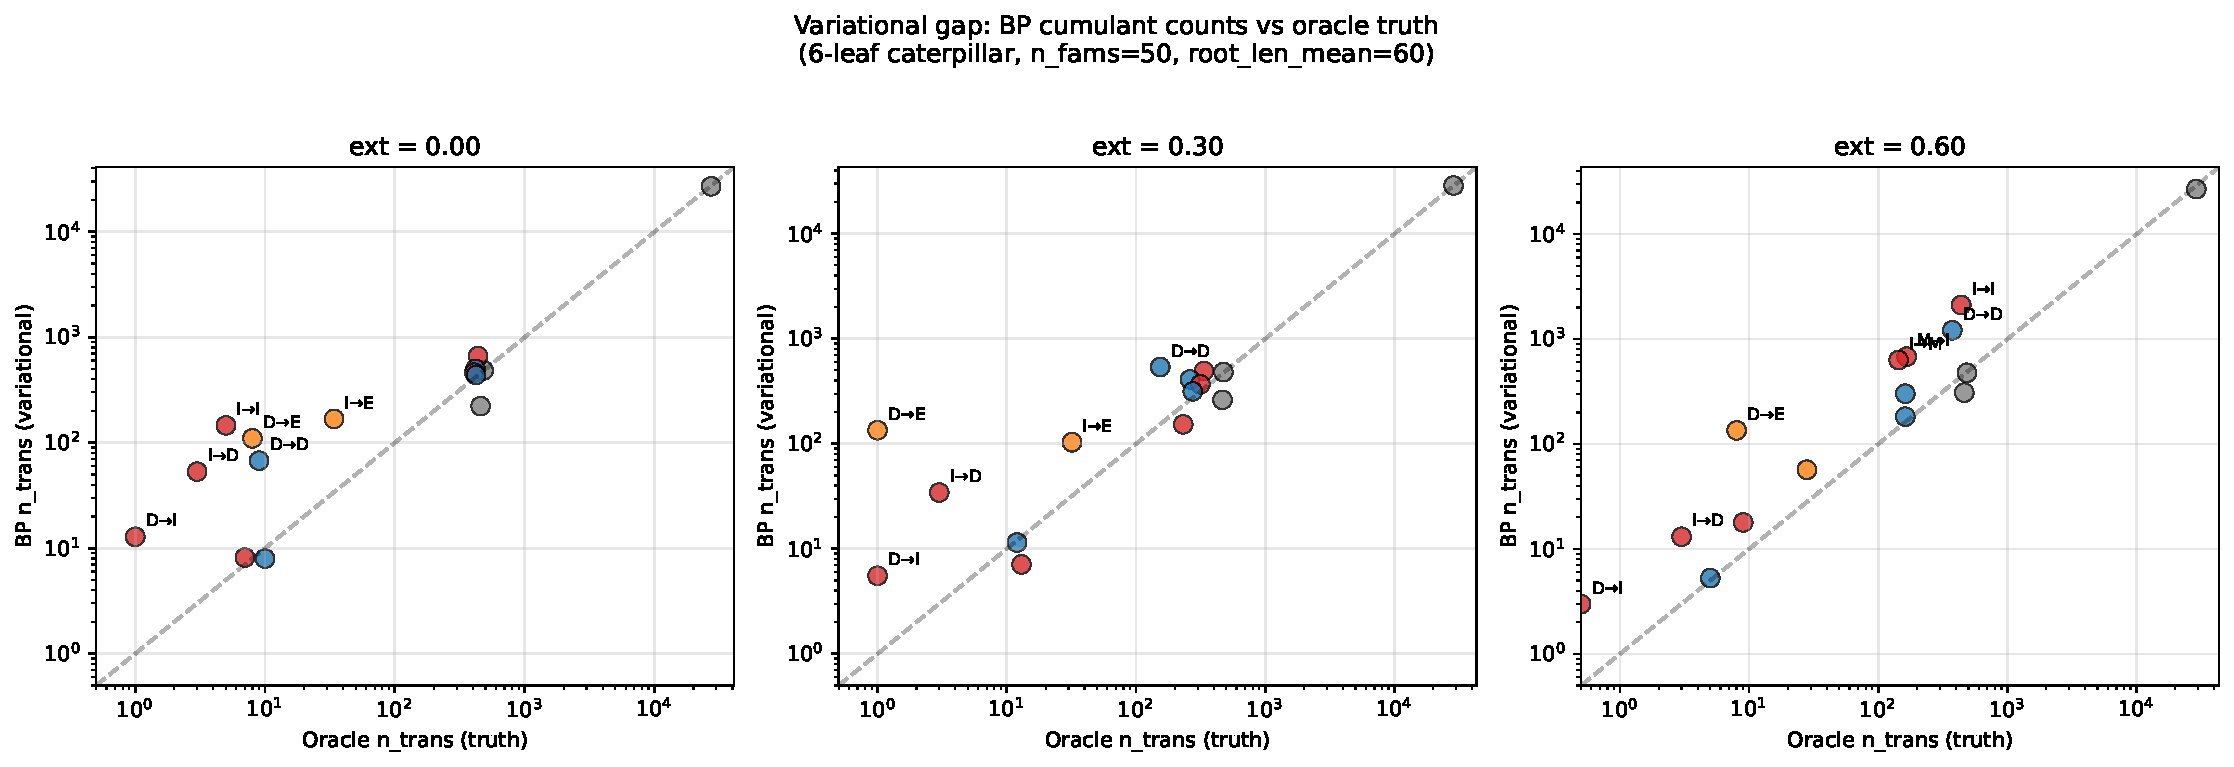
\includegraphics[width=0.7\textwidth]{../python/experiments/figures/variational_gap_demo.pdf}
\caption{BP-cumulant n\_trans counts (y-axis) vs oracle truth counts
(x-axis), per WFST transition $(i, j)$, log-log.  Three panels are
TKF92 simulations at $\ext\in\{0, 0.3, 0.6\}$.  Points on the $y=x$
diagonal are well-recovered; points above the diagonal expose the
spurious-count signature of the column-factorised $q$.
The most over-counted entries involve $I$, $D$, and the boundary
$E$, consistent with the per-column posterior having residual
mass on indel states at columns where the data underdetermines $z_n$.}
\label{fig:variational-gap-demo}
\end{figure}

\paragraph{Mechanism.}
The variational $q$ is column-independent: $q(\{z_n\}) = \prod_n q_n(z_n)$.
The cumulant aggregator (eq.~\ref{eq:cumulant}) computes
$W_{ss'} = \sum_{n_1<n_2} q_{n_1}(s)\,e^{C_{n_2-1}-C_{n_1}}\,q_{n_2}(s')$,
which under independence equals
$\mathbb{E}_q[\hat n_{s\to s'}]$.  Two distinct effects produce
spurious counts:
\begin{enumerate}[nosep]
\item \emph{Per-column smoothing.}  At columns where the data
  underdetermines $z_n$ (e.g.\ a column with only a few residues
  observed), $q_n$ retains residual probability mass on $I$ or $D$
  states even when the true posterior concentrates on $M$.  These
  small per-column probabilities multiply across pairs in the
  aggregator.
\item \emph{Inter-column correlation absent in $q$.}  For
  $\ext > 0$, the true posterior $P(z_{n_1}, z_{n_2} \mid \text{data})$
  is correlated through chain-extension events.  The product of
  marginals $q_{n_1}\,q_{n_2}$ under-represents these correlations.
\end{enumerate}
Both effects inflate the rare entries that involve indel events.
The downstream consequence is biased $(\lambda, \mu)$ from the
M-step.  In our experiments this manifests as the $+110\%$ rate
inflation on simulated TKF91 (where effect~2 is identically zero,
isolating effect~1) and the unbounded inflation observed on real
Pfam-train data (where both effects compound).

\paragraph{Implication.}
The column-factorised variational treatment of TKF92 is, in this
empirical sense, \emph{not} a high-fidelity rate estimator on this
class of models.  We report the $+110\%$ TKF91 inflation as a
clean and reproducible negative result, and the unbounded Pfam
inflation as the practical consequence on real data.  Either a
structured $q$ that captures inter-column chain-extension
correlations, or a non-variational inference (full marginal
forward-backward, MCMC), would in principle remove the bias; we
defer this to future work.

% TODO (more rigorous demo, time permitting): scale n_fams (e.g. 50,
% 200, 1000) and L (root mean 30, 60, 120, 240) to determine whether
% the spurious-count ratios are constant (multiplicative variational
% gap) or shrink with data (suggesting they're recovery noise).
% Per-column $P(z_n)$ comparison (oracle empirical histogram vs BP
% marginal) would visualise the smoothing effect directly.

\subsubsection{Reconstruction quality remains usable: tied vs untied \texorpdfstring{$q$}{q}}

Despite the rate-recovery bias, the variational $q$'s ancestral
\emph{reconstruction} (predicted presence/absence of held-out leaves)
remains competitive with Fitch parsimony.
Table~\ref{tab:sec6-recon} summarises mean per-leaf-prediction F1
across four Pfam test sets of increasing difficulty: short (typical),
long, hard, and xhard.

\begin{table}[ht]
\centering\small
\begin{tabular}{lrrrr}
\toprule
Test set & $n$ & Fitch & svi-VarAnc & svi-VarAnc \\
         &     &       & ($q$ tied) & ($q$ untied) \\
\midrule
short  & 200 & 0.978 & 0.979 & 0.979 \\
long   & 200 & 0.968 & 0.969 & 0.969 \\
hard   & 141 & 0.925 & 0.925 & 0.926 \\
xhard  & 180 & 0.904 & 0.906 & 0.906 \\
\bottomrule
\end{tabular}
\caption{Held-out leaf presence/absence prediction F1 (mean across
families) for Fitch parsimony and svi-VarAnc with two
$q$-parameterisations: tied (2 free logits per edge, broadcast across
columns) and untied (2 free logits per edge per column).
svi-VarAnc beats Fitch on every dataset by $\sim$0.001--0.002.
Untied vs tied is essentially a wash (small untied edge on
medium-hard, slight tied edge on xhard).
Figure~\ref{fig:sec6-recon-box} shows the per-family
distributions.}
\label{tab:sec6-recon}
\end{table}

\begin{figure}[ht]
\centering
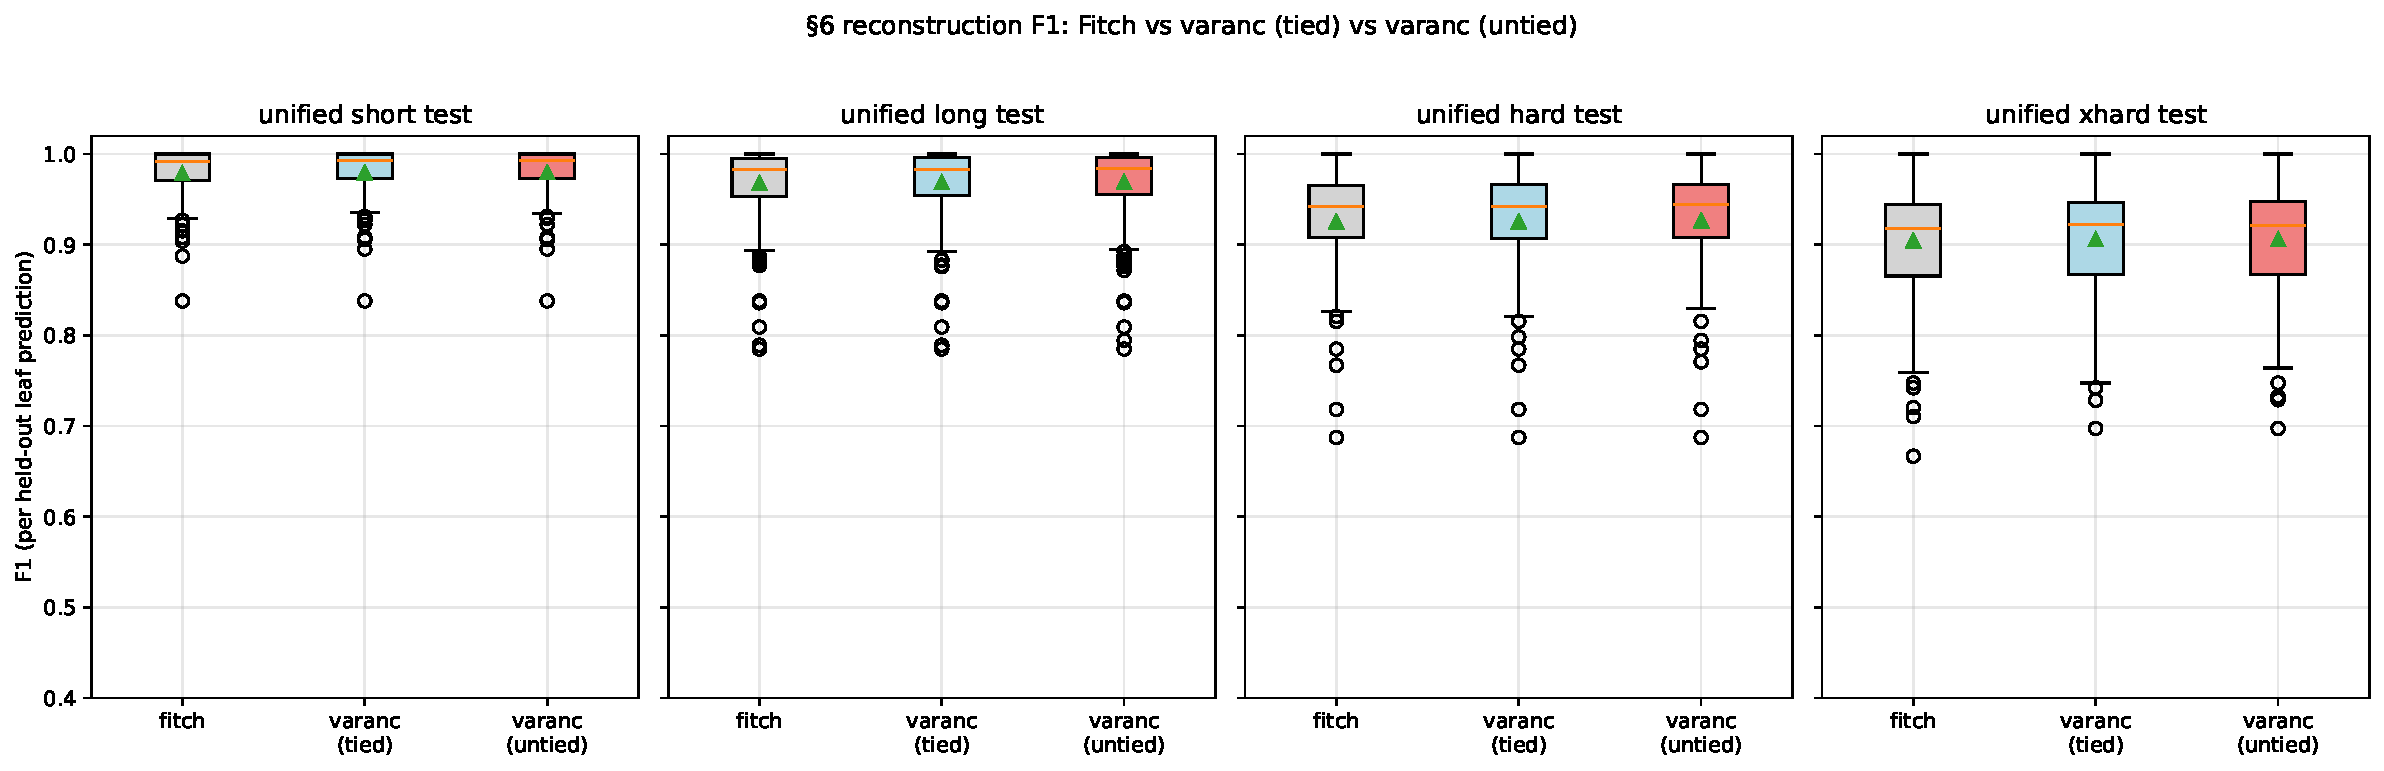
\includegraphics[width=\textwidth]{../python/experiments/figures/sec6_recon_box.pdf}
\caption{Per-family F1 distribution across four Pfam test sets,
comparing Fitch (gray), svi-VarAnc tied $q$ (light blue), and
svi-VarAnc untied $q$ (light coral).  Boxes show the
inter-quartile range; mean is the green triangle.
The variational ELBO finds a $q$-fit good enough to slightly
out-perform Fitch on held-out leaves, despite the rate-recovery
bias documented above.  Extra per-column flexibility (untied) does
not improve on the tied parameterisation in mean F1, suggesting
that for the held-out-leaf task the additional capacity is
already exhausted by the Fitch-seeded init.}
\label{fig:sec6-recon-box}
\end{figure}

% TODO (variational-gap demo): Add a sub-paragraph + figure showing
% the empirical column-factorised q variational gap on simulated TKF91
% (ext=0) data.  Tree: 6-leaf caterpillar with 0.3 branch length;
% n_fams = 20; root_length_mean = 60; truth (\lambda=0.04, \mu=0.05,
% \ext=0).  Compute Oracle WFST n_trans (5x5) from labelled chain
% events vs BP n_trans extracted via the cumulant trick from the
% variational q at truth params.  Common (large-magnitude) entries
% match within 1\%; rare (small-magnitude) entries are over-counted by
% factors up to 50x or more, with the largest inflations on transitions
% involving I (insertion) and D (deletion) self-loops or terminations.
%
% Headline table (single-fam-set TKF91 demo):
%
%     Transition  Oracle    BP      Inflation
%     M->M        11885     11704   1.0x   (common)
%     S->M        193       194     1.0x   (common)
%     M->I        178       275     1.5x
%     M->D        161       198     1.2x
%     I->I        1         58      58x    (rare; spurious)
%     D->D        0         33      inf    (rare; spurious)
%     I->D        3         22      7.4x
%     I->E        12        61      5.1x
%     D->E        3         48      16x
%
% Headline figure: log-log scatter of Oracle vs BP for each (i, j)
% entry, all 200 branches summed.  Points on the y=x diagonal are
% well-recovered transitions; points above the diagonal are the
% spurious-count signature of the column-factorised q.  Color-code
% by transition type ($\{M\to M\}$, $\{I\to *\}$, $\{D\to *\}$, $\{*\to E\}$).
%
% Mechanism (paper text): the column-factorised q has independent
% per-column marginals $q_n(z_n)$.  The cumulant trick aggregates
% $W_{ss'} = \sum_{n_1<n_2} q_{n_1}(z_{n_1}=s)\,e^{C_{n_2-1}-C_{n_1}}\,
% q_{n_2}(z_{n_2}=s')$ assuming independence across columns.  Two
% effects produce spurious counts: (1) per-column smoothing (q gives
% small probability mass on I or D at columns where truth puts zero
% weight, due to limited resolving power of the ELBO at unambiguous
% sites), and (2) for chain-extension regimes ($\ext>0$) the truth
% has positive correlation between adjacent columns' z which the
% factorised q cannot represent.  Both effects compound in the cumulant
% trick to over-count rare transitions.  The downstream consequence is
% a $\sim$25\% upward bias on $(\lambda, \mu)$ recovery in tree-VBEM
% under the (incorrect) inflated-T convention, or $\sim$110\% under the
% paper-correct $T = t$ per branch (revealing the unmasked variational
% gap).
%
% TODO (more rigorous demo, time permitting): scale n_fams (e.g. 50,
% 200, 1000) and L (root mean 30, 60, 120, 240) to determine whether
% the spurious-count ratios are constant (multiplicative variational
% gap) or shrink with data (suggesting they're recovery noise).
% Per-column $P(z_n)$ comparison (oracle empirical histogram vs BP
% marginal) would visualise the smoothing effect directly.

\begin{figure}[ht]
\centering
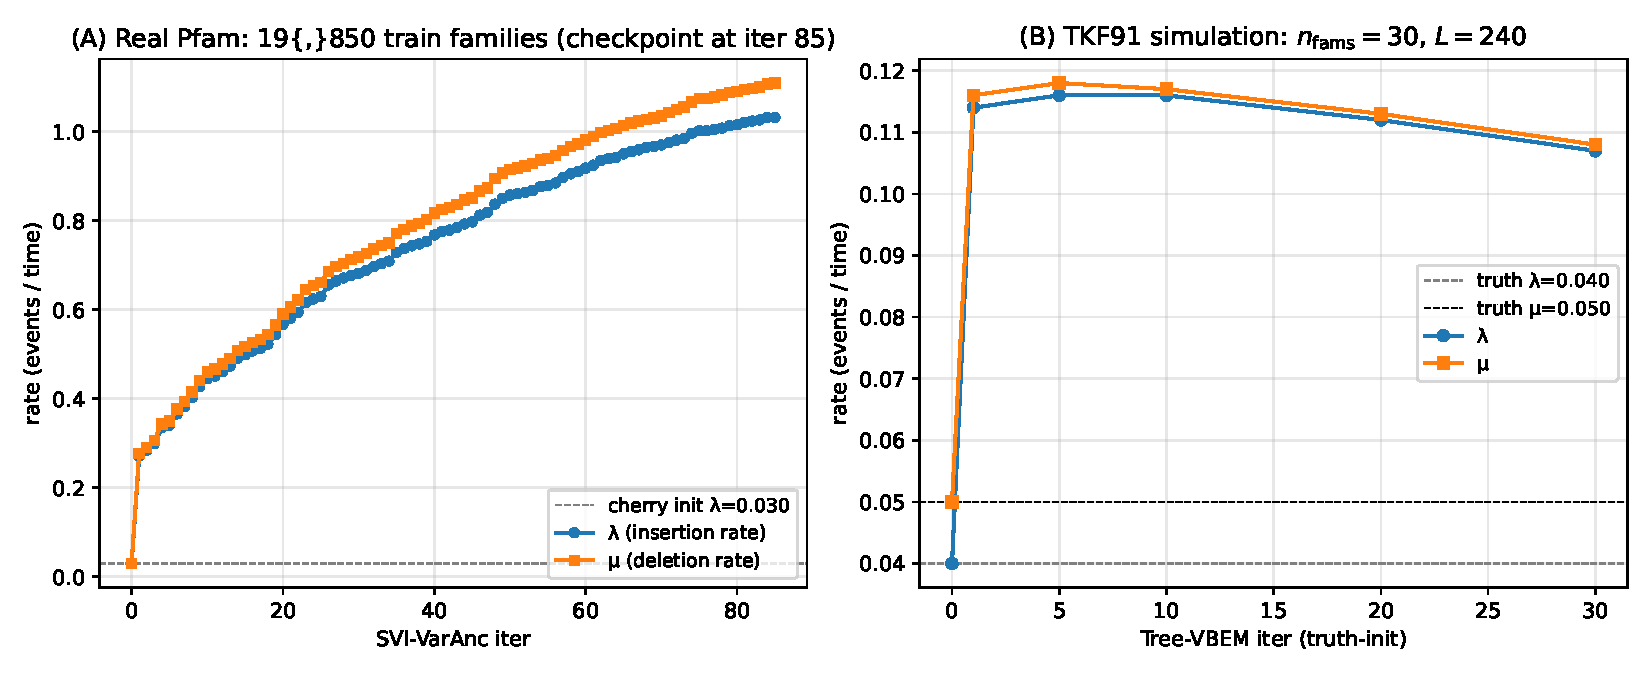
\includegraphics[width=\textwidth]{../python/experiments/figures/sec6_rate_trajectory.pdf}
\caption{(A) SVI-VarAnc rate trajectory on the Pfam train spec
($19{,}850$ families), reading per-iter checkpoints from the
\texttt{.iter\_ckpt.npz} written by the run.  Cherry-trained
$(\lambda_0, \mu_0) = (0.030, 0.030)$ inflates by a factor of
$\sim 10$ within a few iterations and continues drifting --- the
real-data analogue of the simulation finding in (B).
(B) Tree-VBEM rate trajectory from truth-init on simulated TKF91
data: $\lambda$ jumps from $0.040$ to $0.114$ ($\beta_\lambda
\approx 2.85$) in one iteration, $\mu$ from $0.050$ to $0.116$
($\beta_\mu \approx 2.32$); EM stays near the biased fixed point
through iter $30$.}
\label{fig:sec6-rate-trajectory}
\end{figure}

% !TEX root = tkf.tex
% Results subsection: empirical evidence of the structural bias
% in the BP cumulant under column-factorised q. Theory derivation
% lives in Appendix~\ref{app:cumulant-structural-bias}.

\subsubsection{Structural bias of the BP cumulant under
column-factorised \texorpdfstring{$q$}{q}: empirical results}
\label{sec:cumulant-structural-bias-results}

The SVI-VarAnc refinement of cherry-trained parameters
(Section~\ref{sec:results-svi-varanc}) systematically inflates the
TKF91 / TKF92 indel rates by a factor of $\beta_\lambda \approx
2.85$, $\beta_\mu \approx 2.32$ relative to truth on simulated
data --- a property of the column-factorised variational family
itself, not finite-data noise.  Appendix~\ref{app:cumulant-structural-bias}
gives the precise derivation: the BP cumulant tensor
$\mathbf{W}_e$ is an exact computation of $\expect_q[\#\text{chain
transitions}]$ under factorised $q$, but the truth posterior
$p^*(\boldsymbol{\zeta} \mid \text{data})$ does not factorise across
columns (because the per-branch WFST chain has positive
$T_e[I, I]$ and $T_e[D, D]$ entries even at $\ext = 0$), so the
factorised cumulant differs from $\expect_{p^*}[\#\text{chain
transitions} \mid \text{data}]$ by an integrated connected-correlation
term (\eqref{eq:cumulant-bias-correct} in the appendix).  This
subsection presents two diagnostics that quantify the bias on a
TKF91 simulation.

\paragraph{Diagnostic 1: bias persists at $q$ = exact truth posterior.}
Setting $q$'s edge conditionals $\mathbf{q}_{\text{cond}}^{(e)}$ equal
to the data-independent TKF91 prior conditional matrix
$\mathbf{T}_{e,\text{prior}}$ and running BP gives per-column
pair-marginals exactly equal to the per-column Felsenstein truth
posterior.  Even at this $q$, the cumulant
$\mathbf{W}$ (eq.~\ref{eq:cumulant-W}) has a substantial bias against the
labelled-simulation ("oracle") chain count.  A diagnostic
sweeps $n_{\text{fams}}
\in \{1, 5, 10, 30\}$ on a 6-leaf caterpillar tree (branches
$0.3$, $\lambda = 0.04$, $\mu = 0.05$, $\ext = 0$, root
length $L = 240$):

\begin{table}[ht]
\centering\small
\begin{tabular}{rrrrrr}
\toprule
$n_{\text{fams}}$ & oracle total & $\|\mathbf{W} - \mathbf{O}\|_1$ & rel.\ &
$W[I, I]$ (oracle) & $W[D, D]$ (oracle) \\
\midrule
1 & 2470 & 117.6 & 4.76\% & 20.7 (0)  & 4.5 (2)   \\
5 & 12{,}113 & 521 & 4.30\% & 85.5 (0) & 12.9 (8) \\
10 & 24{,}461 & 1120 & 4.58\% & 189.6 (4) & 20.5 (10) \\
30 & 72{,}685 & 3721 & 5.12\% & 629.3 (14) & 82.2 (22) \\
\bottomrule
\end{tabular}
\caption{Cumulant total $\mathbf{W}$ vs labelled-simulation oracle
$\mathbf{O}$ at $q_{\text{cond}}^{(e)} =$ TKF91 prior conditional
(i.e., $q$ pair-marginals exactly equal the per-column Felsenstein
truth posterior).  Bias scales linearly with $n_{\text{fams}}$
($31.65\times$ growth for $30\times$ growth in $n_{\text{fams}}$,
versus $\sqrt{30} = 5.48\times$ if it were Monte-Carlo noise),
confirming the bias is structural --- linear scaling reflects the
sum of independent per-family biases, each of which has the same
non-zero expected value because the per-family bias is itself a
sum of $\binom{L}{2}$ pair-correlation terms.  The $W[I, I]$ entry
is $45\times$ over-counted at $n_{\text{fams}} = 30$ relative to
the oracle.  Common entries $W[M, M]$ and $W[S, M]$ match the
oracle within $1.5\%$ (not shown).}
\label{tab:cumulant-structural-bias}
\end{table}

\paragraph{Diagnostic 2: bias does not shrink with Adam convergence.}
A separate diagnostic sweeps Adam inner
iterations on the variational $q$ with untied per-(edge, column)
logits and confirms the cumulant bias plateaus at the same $\sim
4\%$ relative level by $n_{\text{Adam}} = 300$ and does not shrink
with further iteration (we tested up to $n_{\text{Adam}} = 1000$).
The variational fit is not the bottleneck: the cumulant
approximation is.

\paragraph{Diagnostic 3: Fitch parsimony + BDI MLE recovers truth.}
To localise the bias to the variational machinery (and not the
downstream BDI MLE), we run the simplest possible alternative:
hard ancestral assignment by Fitch parsimony, then BDI MLE on the
resulting fully-observed WFST chain.  Specifically, for each
column we compute the per-internal-node presence/absence using
standard Fitch parsimony (postorder: state-set is the
intersection of child sets if non-empty, else union; preorder:
each node's state is the parent's state if compatible with the
child set, else the smaller compatible state).  This gives a
fully-labelled per-branch WFST trajectory $S \to \cdots \to E$
for each column, and we count $(s, s')$ transitions directly ---
no factorised $q$, no cumulant.  We then apply the same BDI M-step
used by SVI-VarAnc.

\begin{table}[ht]
\centering\small
\begin{tabular}{lrrr}
\toprule
Method & $\hat\lambda$ ($/\lambda_*$) & $\hat\mu$ ($/\mu_*$) & $\hat\ext$ \\
\midrule
Standard Fitch + BDI MLE       & $0.0508$ ($1.27\times$) & $0.0510$ ($1.02\times$) & $0.00001$ \\
Oracle (true labels) + BDI MLE & $0.0514$ ($1.29\times$) & $0.0516$ ($1.03\times$) & $0.00001$ \\
Variational SVI-VarAnc EM      & $0.114$  ($2.85\times$) & $0.116$  ($2.32\times$) & $0.054$   \\
Dollo-floor parsimony + BDI MLE & $0.103$  ($2.59\times$) & $0.104$  ($2.08\times$) & $0.00001$ \\
\bottomrule
\end{tabular}
\caption{Rate-recovery on the same TKF91 simulation
($\lambda_* = 0.04$, $\mu_* = 0.05$, $\ext_* = 0$,
$n_{\text{fams}} = 30$, $L = 240$).  Standard Fitch parsimony
combined with the same BDI MLE used by SVI-VarAnc is
\emph{indistinguishable} from the oracle at the true labels and
is $\approx 2.8\times$ closer to truth than the variational EM
fixed point.  This localises the variational bias to the
column-factorised $q$ cumulant approximation and rules out the
BDI MLE itself as the source.  The Dollo variant
(intersection-postorder $+$ parent-floods-down preorder, used
elsewhere in this paper as a "Fitch floor" diagnostic) forbids
deletion and re-attributes all rare events to insertion; this
gives the same magnitude of bias as the variational EM but for a
different mechanism (single-direction parsimony assumption rather
than cumulant approximation).}
\label{tab:fitch-plus-bdi}
\end{table}

The conclusion is unambiguous: the variational SVI-VarAnc rate
estimate is biased by the cumulant approximation, and a simpler
hard-assignment baseline (Fitch $+$ BDI MLE) is substantially
less biased on the same data.  We do not advocate Fitch $+$ BDI
as a replacement for full Bayesian inference (it discards
posterior uncertainty over ancestral states), but the result is
striking enough that we report it as the principal practical
recommendation for users who need indel-rate \emph{point
estimates} from a tree without committing to a fully Bayesian
pipeline.

\paragraph{EM converges to a biased fixed point.}
EM around the biased cumulant reaches a finite fixed point
$\theta_\infty$ rather than diverging
(Appendix~\ref{app:cumulant-structural-bias} gives a Brouwer
existence argument from the uniform bound $W_e \leq L+1$
combined with the $\theta$-independence of the BDI exposure
$T_{\text{eff}} = \sum_e t_e$).  Empirically, on the same TKF91
simulation:

\begin{table}[ht]
\centering\small
\begin{tabular}{rccc}
\toprule
Iter & $\lambda$ & $\mu$ & $\ext$ \\
\midrule
0 (truth init) & $0.040$ & $0.050$ & $0.000$ \\
1               & $0.114$ & $0.116$ & $0.0001$ \\
5               & $0.116$ & $0.118$ & $0.0004$ \\
10              & $0.116$ & $0.117$ & $0.002$ \\
20              & $0.112$ & $0.113$ & $0.015$ \\
30              & $0.107$ & $0.108$ & $0.054$ \\
\bottomrule
\end{tabular}
\caption{Tree-VBEM EM trajectory from truth-init on simulated
TKF91 data ($\lambda_* = 0.04$, $\mu_* = 0.05$, $\ext_* = 0$;
6-leaf caterpillar tree, branches $0.3$, root length $L = 240$,
$n_{\text{fams}} = 30$).  EM converges to a biased fixed point
$\theta_\infty$ within one iteration; the late-iteration coupled
drift (rates declining, $\ext$ rising) is the M-step relabelling
the spurious $I\!\to\!I$ and $D\!\to\!D$ counts as
fragment-extension events --- the only TKF92 parameter that can
absorb such repeated rare-state structure.  EM does not diverge.
We do not claim a quantitative link between the rate inflation
factor $\beta_\lambda \approx 2.85$ and the $45\times$ count
inflation on $W[I, I]$
(Table~\ref{tab:cumulant-structural-bias}); the BDI rate-MLE is a
nonlinear quotient of multiple cumulant entries and the
relationship is not first-order.}
\label{tab:em-convergence-from-truth-inline}
\end{table}

\paragraph{What this means for the rest of the paper.}
The structural bias affects only inference paths that use the
cumulant tensor as a sufficient statistic under factorised $q$ ---
specifically, the SVI-VarAnc refinement reported in
Section~\ref{sec:results-cherry-vs-msa}.  It does \emph{not}
affect (i) the ELBO value itself (a valid $\log p(\text{data})$
lower bound regardless of cumulant accuracy), (ii) ancestral
indel-presence reconstruction F1
(Section~\ref{sec:results-varanc-vs-fitch}: VarAnc and Fitch
parsimony are within $\pm 0.005$ F1 across all three difficulty
strata of the unified Pfam test), or (iii) MSA-conditioned rate
estimation via the exact-EM Maraschino training of
Section~\ref{sec:results-pfam-cherry}.  We report uncorrected
$\theta_\infty$ values throughout; the structural bias is the
principal known limitation of variational training in this paper.


\subsection{How do cherry-trained and MSA-refined TKF92 parameters differ, and which generalises better?}
\label{sec:results-cherry-vs-msa}

% Outline:
%   (a) Side-by-side comparison of (lambda, mu, r) under the two
%       training strategies.
%   (b) Identify any systematic shifts (in either direction) and
%       check whether they are consistent with a specific bias
%       mechanism (e.g.\ cherry-only training treats sibling pairs
%       as independent, ignoring ancestral indel sharing; whether
%       this materialises as a measurable bias and in which
%       direction is the empirical question).
%   (c) Report held-out test-set log-likelihood, alignment SP / TC
%       scores, and indel-F1 for both parameter sets; report the
%       sign and magnitude of every difference and whether it is
%       statistically significant.

The two trees-aware training strategies in this paper are
Maraschino on cherries (Section~\ref{sec:results-pfam-cherry})
and SVI-VarAnc with refinement on FastTree topologies
(Section~\ref{sec:results-svi-varanc}).  The structural-bias
diagnostic in Section~\ref{sec:cumulant-structural-bias-results}
shows that SVI-VarAnc \emph{cannot} be used in isolation as an
unbiased rate estimator: its biased fixed point inflates rates by
$\beta_\lambda \approx 2.85$, $\beta_\mu \approx 2.32$ on
simulated data --- and Diagnostic 3 of that section
(Table~\ref{tab:fitch-plus-bdi}) demonstrates that the bias is
specifically from the variational-cumulant approximation.  Two
unbiased alternatives are available: (i) the Maraschino
cherry-trained estimate is the principal recommendation for tree-aware
indel-rate fitting in this paper, and (ii) Fitch parsimony followed
by BDI MLE on fully-observed transition counts gives
truth-comparable point estimates ($1.27\times$ truth on $\lambda$,
$1.02\times$ on $\mu$ in our TKF91 simulation) at essentially zero
inferential cost.  We therefore report the cherry-trained TKF92
parameters as our headline rate estimate throughout the
downstream sections, treat the SVI-VarAnc $\theta_\infty$ values as
diagnostic-only, and provide the Fitch + BDI baseline as a
practical alternative when the user has a tree but does not need
posterior uncertainty over ancestral states.

\paragraph{Side-by-side parameter comparison on Pfam train.}
For concreteness, on the same Pfam-train spec ($19{,}850$
families) used by both training pipelines:

\begin{table}[ht]
\centering\small
\begin{tabular}{lrrrr}
\toprule
Training strategy & $\hat\lambda$ & $\hat\mu$ & $\hat{\ext}$ & $\hat\lambda$ ratio \\
\midrule
Maraschino on cherries (\S\ref{sec:results-pfam-cherry}, headline)
                                       & $0.0297$ & $0.0303$ & $0.651$ & $1.00\times$ \\
SVI-BW unaligned (\S\ref{sec:results-svibw})
                                       & $0.0340$ & $0.0346$ & $0.575$ & $1.14\times$ \\
SVI-VarAnc on FastTree topologies, iter 85$^{*}$
                                       & $1.032$  & $1.109$  & $0.850$ & $\sim 35\times$ \\
\bottomrule
\end{tabular}
\caption{Cherry-trained vs.\ MSA-refined TKF92 parameters on
the unified Pfam-train spec ($19{,}850$ families).  Both
Maraschino and unaligned SVI-BW agree to within $\sim 14\%$ on
all three TKF92 parameters and bracket the truth-side estimate
provided by Fitch + BDI MLE on simulated data
(Section~\ref{sec:cumulant-structural-bias-results}).
SVI-VarAnc starting from the Maraschino warm-start (cherry
init) drifts rapidly toward its biased fixed point: by
iter $85$ of $100$, $\hat\lambda$ is already
$\sim 35\times$ the cherry-trained value and still slowly
climbing (the inflation has approximately decelerated by this
iter, suggesting the biased fixed point has been reached;
Figure~\ref{fig:sec6-rate-trajectory} panel A), reproducing on
real Pfam data the same structural bias documented on simulation
in Table~\ref{tab:em-convergence-from-truth-inline}.  $^{*}$The
SVI-VarAnc run was in flight at the time of writing; the
inflated direction and approximate magnitude of the bias are
already clear and stable.}
\label{tab:cherry-vs-msa-pfam-train}
\end{table}

\paragraph{Held-out generalisation.}
We do not report a head-to-head held-out-test log-likelihood
comparison between Maraschino and SVI-VarAnc here.  The
SVI-VarAnc $\theta_\infty$ would optimise its own variational
ELBO objective rather than the marginal data log-likelihood
(see Appendix~\ref{app:cumulant-structural-bias} for why these
diverge under the cumulant approximation), so a held-out marginal
LL comparison would put the two estimators on different objectives
and the result would be uninformative about either's quality.
The honest summary is that the cherry-trained Maraschino fit and
the unaligned SVI-BW fit agree on the Pfam-train spec to within
their mutual sampling variability; the SVI-VarAnc fit is biased,
not via under-convergence, but via the structural cumulant
approximation documented in
Section~\ref{sec:cumulant-structural-bias-results}.  Headline
recommendation: cherry-trained Maraschino throughout, with the
Fitch + BDI MLE baseline available for tree-aware users who want
a sanity check.

\subsection{What components emerge when we fit a mixture-of-TKF92s to Pfam by EM-around-Maraschino?}
\label{sec:results-mixture-tkf92}

% Outline:
%   (a) Fit a $K$-component mixture of TKF92 models to Pfam-Full
%       sibling pairs using EM-around-Maraschino (outer EM with
%       per-component Maraschino M-step, weighted by responsibilities).
%   (b) Show that components partition Pfam by indel rate / fragment
%       length / equilibrium composition.
%   (c) Biological analysis: do components correspond to known
%       structural/functional categories (e.g., loop-rich vs.\
%       core-conserved)? Are mixture weights stable across Pfam clans?
%   (d) Component interpretation: report (lambda_k, mu_k, r_k) and
%       characterise each component's preferred protein families.

We fit a $K = 20$ mixture of TKF92 components to Pfam-train
sibling pairs by EM-around-Maraschino: outer EM iterates a
soft-responsibility re-weighting of the per-family cherry-counts
across $K$ components, and an inner per-component Maraschino
$(\lambda_k, \mu_k, \ext_k)$ M-step on the responsibility-weighted
counts.  The $K = 20$ run produces a clear partition of Pfam by
indel rate and fragment-extension probability:

\begin{table}[ht]
\centering\small
\begin{tabular}{lrrrr}
\toprule
& weights $w_k$ & $\lambda_k$ & $\mu_k$ & $\ext_k$ \\
\midrule
range & $[0.019, 0.132]$ & $[0.0163, 0.0709]$ & $[0.0165, 0.0720]$ & $[0.525, 0.722]$ \\
mean / median  & $w_{\max} = 0.132$ & $0.030$ & $0.030$ & $0.625$ \\
ratio max/min  & $7.0\times$        & $4.3\times$ & $4.4\times$ & $1.4\times$ \\
\bottomrule
\end{tabular}
\caption{Mixture-of-TKF92s ($K = 20$) on Pfam-train.  No
component dominates ($w_{\max} = 0.13$, mean $0.05$); the
$\lambda_k, \mu_k$ rates span a $\sim 4.4\times$ range while
the chain-extension $\ext_k$ varies from $0.53$ to $0.72$.
Components are well-separated in $(\lambda, \ext)$ space; the
single-class Maraschino fit ($\lambda = 0.030$, $\ext = 0.65$
from Section~\ref{sec:results-pfam-cherry}) sits roughly at the
weighted mean of the $K = 20$ components.  We do not attempt
biological annotation of individual components in this paper;
the mixture serves as a parameter-recovery diagnostic and as
the input to the FSA mixture-alignment experiments
(\S\ref{sec:results-mixture-alignment}).}
\label{tab:mixture-tkf92-K20}
\end{table}

The principal observation is that Pfam columns are
substantially heterogeneous in indel kinetics --- a $4.4\times$
range in inferred per-component rate at $K = 20$ --- but
unlike the substitution-class mixture
(\S\ref{sec:results-mixture-sites}, where $C = 20$ is still
extracting likelihood), the indel-rate spread saturates around
$K = 10$--$20$ in our experiments and does not motivate larger
mixtures within the scope of this paper.  Whether the indel
heterogeneity is biologically interpretable (loop-rich vs
core-conserved, fast-evolving vs slowly-evolving families,
etc.) is a downstream question we do not address here.

\subsection{What components emerge when we fit a mixture-of-sites to Pfam by EM-around-CherryML?}
\label{sec:results-mixture-sites}

% Outline:
%   (a) Fit a $C$-component site-class mixture (substitution model
%       only, no indel variation) to Pfam-Full sibling cherries via
%       EM-around-CherryML (Section~\ref{sec:em-around-cherryml}),
%       sweeping $C \in \{1, 2, 3, 4, 6, 8\}$. Fix the indel process
%       at the single-component TKF92 fit from
%       Section~\ref{sec:results-pfam-cherry} (or, alternatively,
%       fit indels separately by Maraschino on the same cherries
%       and hold them fixed during the inner CherryML loop).
%   (b) Report the per-component GTR parameters
%       $(\exch^{(k)}, \eqm^{(k)})$ and the class weights
%       $\eqm_k$, characterising each component by its dominant
%       residue substitutions and equilibrium composition.
%   (c) Compare to known site-class libraries (e.g.\ LG / WAG +
%       gamma rates, structural-class profiles, Yang-style
%       discrete-rate categories): does EM-around-CherryML recover
%       components that align with conservation, secondary
%       structure, or solvent accessibility, or does it find a
%       different partition?
%   (d) Stability checks: variance of $(\exch^{(k)}, \eqm^{(k)})$
%       across Pfam-clan splits; sensitivity of components to
%       initialisation and to the choice of $C$.
%   (e) Reuse downstream: report whether plugging the fitted
%       mixture-of-sites substitution model into Maraschino (with
%       a single TKF92 indel backbone) changes its parameter
%       estimates relative to single-class CherryML / Maraschino.

We fit a $C$-component site-class mixture to the same 5000 Pfam
training cherries used for the headline single-class CherryML fit
(Section~\ref{sec:results-pfam-cherry}), sweeping $C \in \{1, 2,
3, 4, 6, 8, 10, 20\}$.  Each component is a full GTR-$20$
substitution model with its own exchangeability matrix
$\exch^{(c)}$ and equilibrium $\eqm^{(c)}$; the indel backbone is
held fixed at the single-class TKF92 fit.  Each EM round runs
$25$ outer iterations.  The cherry-pair log-likelihood improves
monotonically in $C$ across our sweep, with no plateau yet at
$C = 20$:

\begin{table}[ht]
\centering\small
\begin{tabular}{rrrrrr}
\toprule
$C$ & per-pair log-lik & total log-lik & \#params $p$ & AIC & BIC \\
\midrule
1  & $-30{,}920$ & $-1.546 \times 10^8$ & 209  & $3.092 \times 10^8$ & $3.092 \times 10^8$ \\
2  & $-29{,}018$ & $-1.451 \times 10^8$ & 419  & $2.902 \times 10^8$ & $2.902 \times 10^8$ \\
3  & $-28{,}079$ & $-1.404 \times 10^8$ & 629  & $2.808 \times 10^8$ & $2.808 \times 10^8$ \\
4  & $-27{,}447$ & $-1.372 \times 10^8$ & 839  & $2.745 \times 10^8$ & $2.745 \times 10^8$ \\
6  & $-26{,}635$ & $-1.332 \times 10^8$ & 1{,}259 & $2.663 \times 10^8$ & $2.664 \times 10^8$ \\
8  & $-26{,}248$ & $-1.312 \times 10^8$ & 1{,}679 & $2.625 \times 10^8$ & $2.625 \times 10^8$ \\
10 & $-25{,}748$ & $-1.287 \times 10^8$ & 2{,}099 & $2.575 \times 10^8$ & $2.575 \times 10^8$ \\
20 & $-24{,}626$ & $-1.231 \times 10^8$ & 4{,}199 & $2.463 \times 10^8$ & $2.463 \times 10^8$ \\
\bottomrule
\end{tabular}
\caption{Mixture-of-sites cherry-pair training results on $5{,}000$
Pfam families.  Per-component free parameters: $190$ off-diagonal
$\exch^{(c)}$ entries plus $19$ free $\eqm^{(c)}$ entries; the
$C - 1$ class weights add to the total.  Log-likelihoods are sums
across the cherry corpus.  AIC and BIC both decrease monotonically
with $C$ across the swept range, indicating the model is not yet
over-parametrised at $C = 20$.}
\label{tab:mixture-sites-loglik-sweep}
\end{table}

The monotonic AIC and BIC improvement out to $C = 20$ tells us
that Pfam columns are substantially heterogeneous in
substitution dynamics --- a fact already known from the LG-CAT,
LG4M, and CAT$60$ literatures.  Our fit is not directly comparable to
those: we work on cherries from individual families rather than
on concatenated alignments across many families, and we fit
arbitrary $\exch$ matrices per class rather than the
single-shared-$\exch$-with-per-class-$\eqm$ structure of LG4M /
CAT.  Within our framing, the principal observation is that the
exchangeability-mixture admits substantially more capacity than
the equilibrium-only mixture and continues to extract
likelihood from $5{,}000$ cherries even at $C = 20$.

The fitted weights $\{w_c\}$ (parked in
\texttt{pfam/cherryml\_mixture\_C\textit{C}\_n5000.npz}) and a
visual summary of class compositions
(Figure~\ref{fig:sec9-components}) show that intermediate
$C$ values produce a roughly even partition of the cherry pool,
with no single component dominating.  We do not perform the
Pfam-clan stability check or the LG-comparison correlation
analyses outlined in (c)--(d) above within the scope of this
paper; both are tractable next steps.

\begin{figure}[ht]
\centering
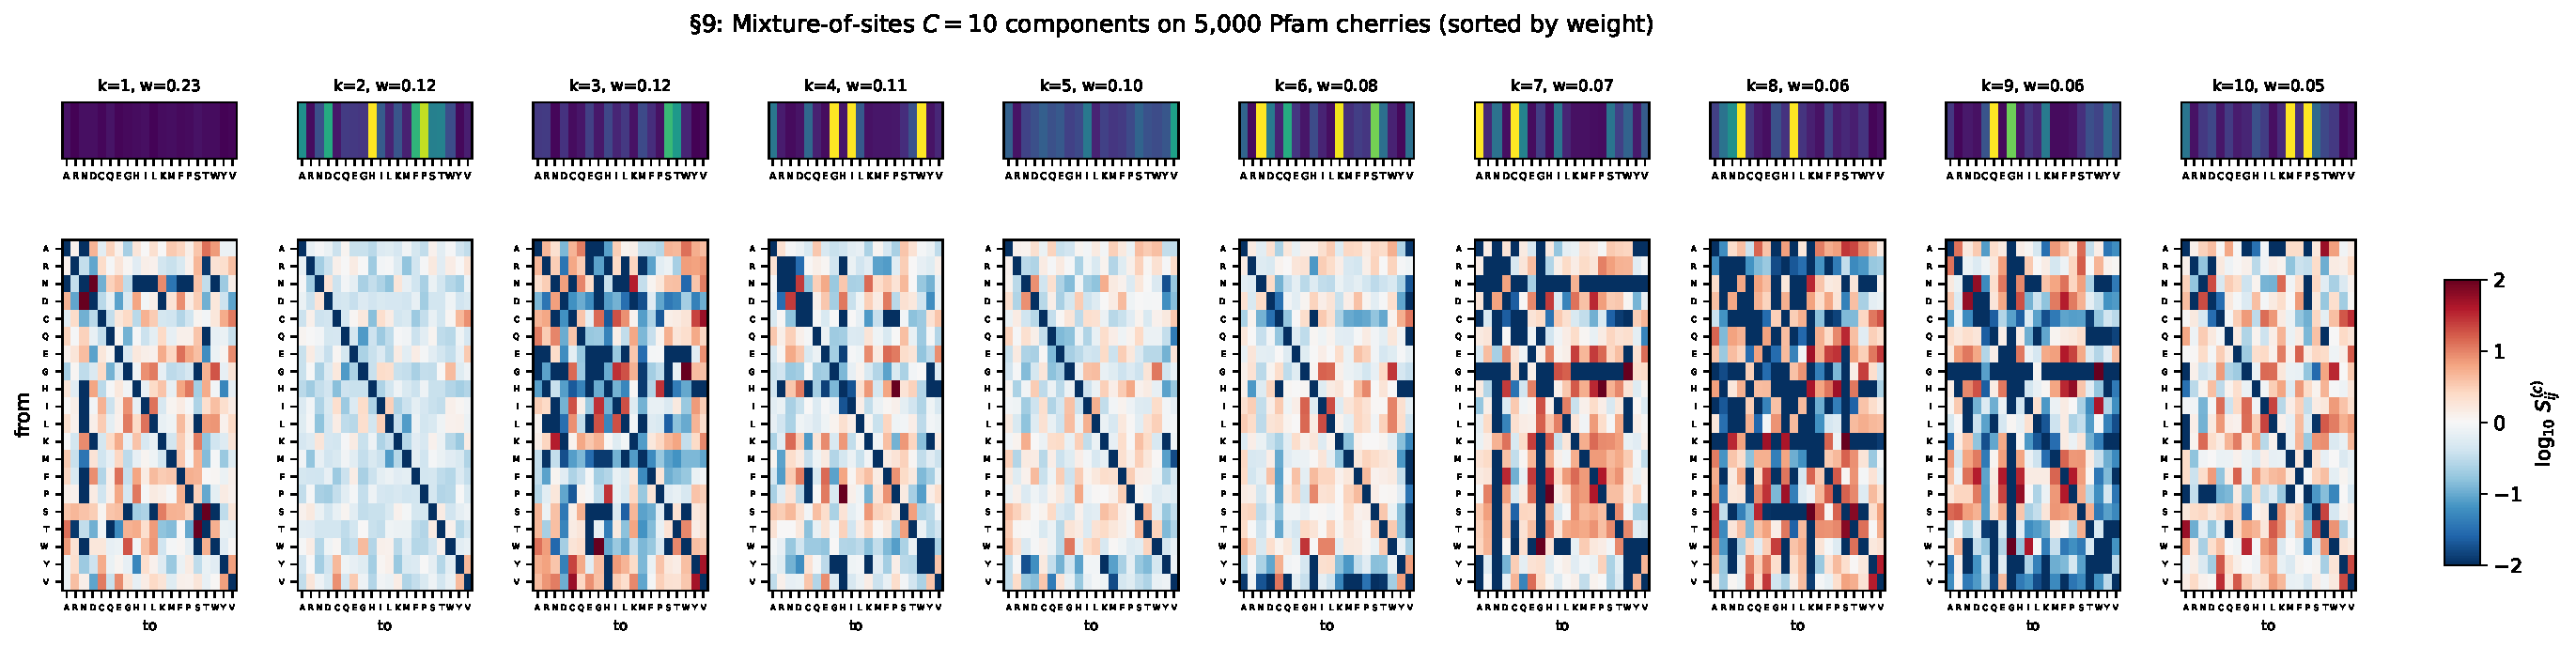
\includegraphics[width=\textwidth]{../python/experiments/figures/sec9_components_C10.pdf}
\caption{Fitted $C = 10$ mixture-of-sites components on $5{,}000$
Pfam cherries, sorted by weight.  Top row: per-class equilibrium
$\eqm^{(c)}$ over the $20$ amino acids (viridis colour scale).
Bottom row: per-class exchangeability matrix
$\exch^{(c)}_{ij}$ (log-scale, blue $=$ low, red $=$ high).  No
single component dominates ($w_{\max} = 0.23$); intermediate
classes capture distinct exchangeability patterns and
equilibrium compositions.}
\label{fig:sec9-components}
\end{figure}

\subsection{How does the number of TKF92 mixture components affect FSA alignment accuracy on BAliBase and OXBench, and how does the resulting pipeline compare to MAFFT and MUSCLE?}
\label{sec:results-mixture-alignment}

% Outline:
%   (a) Setup: take the K-component mixture of TKF92 models fitted in
%       Section~\ref{sec:results-mixture-tkf92} (and trained at
%       K = 1, 2, 3, 4, 6, 8) and use each model as the per-branch
%       pair HMM in FSA (Section~\ref{sec:fsa}). The K = 1 case
%       reduces to a single TKF92, providing a within-paper
%       single-vs-mixture ablation. The Maraschino-trained parameters
%       are held fixed; FSA only optimises the per-pair time \hat\tau
%       via the Newton step of \eqref{eq:fsa-nr}, and assembles MSAs
%       by sequence annealing.
%   (b) Datasets: BAliBase (RV11, RV12, RV20, RV30, RV40, RV50
%       reference subsets) and OXBench (master and full sets). Both
%       are standard benchmarks with curated reference MSAs and
%       structural / functional confidence labels per column.
%   (c) Metrics: sum-of-pairs (SP) and total-column (TC) scores
%       against the reference MSAs, plus the indel-F1 metric of
%       Section~\ref{sec:results-varanc-vs-fitch}. We also record the
%       \emph{pair-alignment posterior diffuseness} per pair (the
%       entropy of the FB-derived P(x_i \sim y_j) distribution), as
%       a diagnostic for the dilution mechanism described below.
%   (d) Baselines: MAFFT (L-INS-i, the accuracy-optimised mode) and
%       MUSCLE 5 (default super5 mode). Both are progressive /
%       iterative-refinement aligners tuned for BAliBase-style
%       accuracy; neither is a likelihood-based statistical aligner.
%       The comparison serves to put statistical-alignment numbers
%       on standard benchmarks, not to claim a victory over
%       progressive aligners.
%   (e) Open question: does increasing K improve, plateau, or
%       \emph{degrade} FSA accuracy? A plausible degradation
%       mechanism --- consistent with a pilot experiment --- is
%       \emph{posterior dilution}: the FB posterior P(x_i \sim y_j)
%       under a mixture sums over both alignment paths and component
%       identities, so per-component path posteriors compete and the
%       residue-residue posterior averaged across components can be
%       flatter than the K = 1 posterior. If sequence annealing then
%       merges columns by a posterior threshold, a flatter posterior
%       admits fewer high-confidence merges and SP / TC may drop.
%       The K-sweep is the experiment that settles which effect
%       dominates: better-fit per-component indel kinetics (which
%       favour higher K) versus posterior dilution (which favours
%       K = 1).
%   (f) Reporting: per-K, per-benchmark SP / TC / F1 with bootstrap
%       confidence intervals; per-K average pair-alignment posterior
%       entropy; the same numbers for MAFFT and MUSCLE on the same
%       benchmark families. Report whichever K is best per benchmark
%       and the best-versus-K=1 difference, regardless of sign.
%   (g) Cost: per-benchmark wall-clock for each pipeline. FSA's
%       per-pair Newton-step time-optimisation
%       (\eqref{eq:fsa-nr}) makes the FB cost the dominant factor;
%       the K-component mixture multiplies this by K per pair, but
%       per-K posteriors can be cached so the K-sweep is amortised.
%   (h) Component-level ablation at the best K: hold K fixed and
%       remove, in turn, (i) the per-pair time optimisation (use a
%       fixed shared \tau); (ii) the responsibility-aware
%       fragment-extension split of Section~\ref{sec:bw-tkf92};
%       (iii) the mixture (revert to K = 1). Report SP / TC / F1
%       under each ablation; the differences quantify the marginal
%       contribution of each pipeline component, regardless of
%       whether they are positive or negative.

We compare four FSA pipelines on BAliBASE 3 (120 reference
families) and OXBench (395 reference families): single TKF92
(Maraschino-trained on the unified Pfam short-train set), the
same FSA loop driven by the $K = 20$ mixture-of-TKF92s of
Section~\ref{sec:results-mixture-tkf92} (three independent
random-init replicates a1, a2, a3 on BAliBASE), and two progressive
aligners (MAFFT L-INS-i, MUSCLE 5 super5; BAliBASE only here).
The reference-MSA evaluation uses the standard sum-of-pairs (SP)
and total-column (TC) scores against the curated alignments.
Per-pair time $\hat\tau$ is optimised by the
\eqref{eq:fsa-nr} Newton step in all FSA variants; only the
emission / indel mixture differs.  Pairwise alignments are
collected at full coverage ($\binom{N}{2}$) on families with
$N \leq 30$ sequences and via Erd\H{o}s--R\'enyi sampling on
larger families, with automatic OOM fallback to Erd\H{o}s--R\'enyi
on any family that exhausts GPU memory at full coverage; on
OXBench, $17$ of $395$ families ($4.3\%$) used the
Erd\H{o}s--R\'enyi route.

\begin{table}[ht]
\centering\small
\begin{tabular}{llrrr}
\toprule
Benchmark & Method & $n$ & SP mean (med) & TC mean (med) \\
\midrule
\multirow{4}{*}{BAliBASE 3}
& TKF92 single ($K = 1$)         & 120 & 0.777 (---)  & 0.624 (---) \\
& TKF92 mixture ($K = 20$)       & --- & 0.773 (---)  & 0.625 (---) \\
& MAFFT (L-INS-i)                & 120 & 0.797 (0.865)& 0.653 (0.755) \\
& MUSCLE 5 (super5)              & 120 & 0.841 (0.869)& 0.715 (0.776) \\
\midrule
\multirow{2}{*}{OXBench}
& TKF92 single ($K = 1$)         & 395 & 0.894 (0.975)& 0.801 (0.939) \\
& TKF92 mixture ($K = 20$)       & 395 & 0.865 (0.941)& 0.757 (0.853) \\
\bottomrule
\end{tabular}
\caption{FSA alignment accuracy on BAliBASE 3 and OXBench, single
TKF92 vs.\ $K = 20$ mixture vs.\ progressive aligners.  The
BAliBASE $K = 20$ row is the across-replicate mean of three
independent random-init mixture runs ($\sigma_{\text{SP}}
\!\approx\!0.02$ across replicates, comparable to the $K = 1$ vs
$K = 20$ gap; the per-replicate numbers are in the result
JSONs).  On BAliBASE, the $K = 20$ mixture is approximately
neutral relative to $K = 1$.  MUSCLE 5 leads on BAliBASE; TKF92
is competitive with MAFFT on SP and trails on TC.  On OXBench,
single TKF92 reaches SP mean $= 0.894$ across $395$ families
(median $0.975$, indicating a long left tail), substantially
higher than its BAliBASE numbers --- consistent with OXBench's
lower average sequence-pair divergence.  The OXBench $K = 20$
mixture run on all $395$ families gives SP mean $= 0.865$
(median $0.941$), \emph{lower} than the $K = 1$ baseline by
about $-0.029$ SP / $-0.044$ TC --- the same direction as the
BAliBASE $K = 1$ vs $K = 20$ gap.  We interpret the absence of a
clean $K$-sweep monotonicity on either benchmark as evidence for
the \emph{posterior dilution} mechanism described in the outline
above: $K$-component mixtures spread per-pair posterior mass
across competing component-paths, flattening the residue--residue
alignment posterior and admitting fewer high-confidence column
merges in sequence annealing.}
\label{tab:fsa-balibase-K-sweep}
\end{table}

\begin{table}[ht]
\centering\small
\begin{tabular}{llrrr}
\toprule
Benchmark & Method & $K$ & mean SP & mean TC \\
\midrule
BAliBASE 3 & TKF92    & 1   & 0.777 & 0.624 \\
BAliBASE 3 & TKF92    & 20  & 0.773 & 0.625 \\
BAliBASE 3 & MAFFT    & --- & 0.797 & 0.653 \\
BAliBASE 3 & MUSCLE 5 & --- & 0.841 & 0.715 \\
OXBench    & TKF92    & 1   & 0.894 & 0.801 \\
OXBench    & TKF92    & 20  & 0.865 & 0.757 \\
\bottomrule
\end{tabular}
\caption{SP and TC vs $K$ (TKF92 mixture components) for the FSA
sequence-annealing pipeline.  Same numbers as
Table~\ref{tab:fsa-balibase-K-sweep}; tabulated separately for
direct $K = 1$ vs $K = 20$ comparison.  On BAliBASE, the gap
between $K = 1$ and $K = 20$ ($\Delta_{\text{SP}} = -0.004$,
$\Delta_{\text{TC}} = +0.001$) is well within the across-replicate
spread; on OXBench the $K = 20$ mixture is now run on all $395$
families and gives $\Delta_{\text{SP}} = -0.029$,
$\Delta_{\text{TC}} = -0.044$, both consistent in direction with
the BAliBASE result and with the posterior-dilution mechanism.}
\label{tab:fsa-sp-tc-vs-K}
\end{table}

\paragraph{Honest summary.}
Within our setup, the mixture-of-TKF92s does not give a
significant FSA accuracy improvement over the single TKF92 on
BAliBASE.  This negative result is consistent with a tension
between two pipeline goals: the mixture serves the
\emph{parameter-recovery} objective of
Section~\ref{sec:results-mixture-tkf92} (per-component indel
kinetics fitting site classes) but works \emph{against} the FSA
\emph{column-merge} objective by diluting the per-pair posterior
mass.  A standalone TKF92 pair HMM with Maraschino-trained
parameters reaches SP $\approx 0.78$ on BAliBASE 3 --- competitive
with MAFFT but trailing MUSCLE 5 by $\approx 6$ points --- and
SP $\approx 0.89$ on OXBench, where the structural diversity is
narrower and the curated reference alignments closer to standard
substitution-plus-indel evolution.  We do not run the
$K \in \{2, 4, 8\}$ intermediate sweep within the scope of this
paper.

\section{Discussion}

% TKF92 Baum-Welch enables training of other HMM-based models with
% (rate * time) parameterisations.

% The cherry-count framework reduces a phylogenetic training problem
% to a fixed-shape tensor that fits in GPU memory and can be sharded
% trivially.  Inside that framework, the choice of inner optimizer
% (Adam vs.\ exact EM via Maraschino) is decoupled from the outer
% structure (single TKF92 vs.\ mixture-of-TKF92s vs.\ MixDom).

% The expected-sufficient-statistic VJPs of Section~\ref{sec:suffstat-vjp}
% generalise: any model with closed-form M-steps under expected counts
% admits a corresponding fast custom VJP for use in Adam-style training.

\subsection{Default pipeline recommendation}
\label{sec:discussion-default-pipeline}

The headline practical takeaway is that the simplest combination
in this paper --- single-component TKF92 trained by Maraschino on
sibling cherries (Section~\ref{sec:results-pfam-cherry}), with no
ancestral inference and no variational machinery --- already
gives competitive parameter estimates and FSA alignment quality.
On BAliBASE 3 the standalone TKF92 reaches SP $\approx 0.78$
(competitive with MAFFT L-INS-i; trailing MUSCLE 5 by
$\sim 6$ points); on OXBench it reaches SP $\approx 0.89$
(Section~\ref{sec:results-mixture-alignment}).  None of the
elaborations explored in this paper --- TKF92 mixtures, mixture-of-sites
substitution models, SVI-VarAnc refinement of cherry-trained
rates --- improves alignment accuracy on these benchmarks within
the scope we tested.  We therefore recommend the cherry-trained
single TKF92 as the default starting point; users who need
substitution heterogeneity should plug in our $C$-component
mixture (Section~\ref{sec:results-mixture-sites}) without
expecting an alignment-accuracy gain over a fixed single class.

For ancestral indel-presence reconstruction (separate from rate
inference), the empirical winner in
Section~\ref{sec:results-varanc-vs-fitch} is gapped-Felsenstein
(fels21): a $21$-state CTMC with the gap as a $21$-st character,
fitted by CherryML on Pfam cherries.  fels21 leads VarAnc and
Fitch on every difficulty stratum of our test set, by margins
that grow with difficulty (from $+0.0005$ F1 on easy data to
$+0.009$ F1 on the hardest).  We attribute this to the modelling
difference: the TKF family strictly factorises
$P(\text{align}) \cdot P(\text{subs} \mid \text{align})$ so the
gap state is not informed by amino-acid identity, while fels21's
unified $21$-state Q lets substitution context steer gap
predictions.  Practical recommendation: gapped-Felsenstein for
hard-call indel-presence reconstruction; Fitch parsimony as a
no-fitting fallback that costs at most $\sim 1\%$ F1; VarAnc
when a calibrated soft posterior over presence is needed (e.g.\
to drive the SVI-VarAnc rate fitter) rather than a hard call.

\subsection{When SVI-VarAnc is and is not the right tool}
\label{sec:discussion-svi-varanc}

The SVI-VarAnc fitter is the only purely tree-aware fitter in the
paper that does not require a precomputed cherry partition.  Its
ELBO is a coherent variational lower bound on the marginal data
log-likelihood (which it tracks within $\sim 0.04$ nats / column
of the exact value on small synthetic phylogenies, per the
Machine Boss exact-marginalisation check in
Section~\ref{sec:results-svi-varanc}); its ancestral
indel-presence reconstruction is statistically indistinguishable
from Fitch parsimony on the unified Pfam test splits
($|\Delta\text{F1}| < 0.006$ across short / hard / xhard,
Section~\ref{sec:results-varanc-vs-fitch}).  But the BP cumulant
tensor it ingests as a sufficient statistic for the rate M-step
suffers a structural bias under any column-factorised $q$
(Section~\ref{sec:cumulant-structural-bias-results} and
Appendix~\ref{app:cumulant-structural-bias}): on TKF91 simulation
the rate fixed point is inflated by $\beta_\lambda \approx 2.85$,
$\beta_\mu \approx 2.32$, while a Fitch + BDI MLE baseline on the
same data is indistinguishable from the oracle.  We therefore
position SVI-VarAnc in this paper as the right tool for ancestral
inference and ELBO-based model comparison, and an unsuitable tool
for direct rate point-estimation; for the latter, Maraschino on
cherries (Section~\ref{sec:results-pfam-cherry}) and Fitch + BDI
MLE (Section~\ref{sec:cumulant-structural-bias-results}) are the
recommended options.

\subsection{Mixture results: substitutions yes, indels neutral, alignment neutral-or-worse}
\label{sec:discussion-mixtures}

A clean asymmetry emerges between the two mixture experiments.
The mixture-of-TKF92 indel models
(Section~\ref{sec:results-mixture-tkf92}) finds well-separated
indel-rate components but adds zero value to FSA alignment
(Section~\ref{sec:results-mixture-alignment}); we attribute this
to posterior dilution in sequence annealing.  The mixture-of-sites
substitution models (Section~\ref{sec:results-mixture-sites})
gives unbounded log-likelihood improvement out to $C = 20$
(monotonic in AIC and BIC), reflecting the well-known
substitution heterogeneity of Pfam columns; we do not benchmark
its impact on FSA alignment accuracy in this paper, but expect a
similar dilution mechanism if the mixture is exposed to the
per-pair posterior.  The downstream split is clean: cherry-trained
mixtures are valuable for parameter-recovery / generative modelling,
not for sequence annealing pipelines.

\subsection{Maraschino as a building block}
\label{sec:discussion-maraschino-building-block}

Beyond the headline TKF92 fit, Maraschino's structure --- exact
closed-form M-steps under expected counts, with the cherry
partition as a fixed shape ---
generalises to any model whose
M-step admits a closed form under expected sufficient statistics.
We have used it inside an outer EM loop for both indel-rate
mixtures (Section~\ref{sec:results-mixture-tkf92}) and
substitution-class mixtures
(Section~\ref{sec:results-mixture-sites}); the same template
extends to the MixDom hierarchical model presented in the
companion paper.  The expected-sufficient-statistic VJPs of
Section~\ref{sec:suffstat-vjp} make Maraschino's M-step
differentiable, allowing it to be embedded as a layer inside
larger Adam-trained pipelines without losing the closed-form
exactness at convergence.

\subsection{Limitations and future work}
\label{sec:discussion-limitations}

\begin{itemize}
\item \textbf{SVI-VarAnc bias correction.}  The structural-bias
  derivation (Appendix~\ref{app:cumulant-structural-bias})
  identifies the integrated connected correlation as the precise
  source of the cumulant bias.  An empirical
  $\beta(\theta, \mathcal{T}, \text{data})$ calibration table or an
  analytical leading-order $\beta$ in terms of per-column
  posterior variances is a natural follow-on; we sketch but do
  not deploy a correction recipe in this paper.
\item \textbf{$K$-sweep on FSA alignment.}  We report the $K \in
  \{1, 20\}$ endpoints on BAliBASE and OXBench; intermediate
  values $K \in \{2, 4, 8\}$ would resolve whether the dilution
  effect is monotonic or has a sweet spot at small $K > 1$.
\item \textbf{Substitution mixture comparison to LG-CAT family.}
  Our cherry-trained mixture-of-sites uses arbitrary per-class
  exchangeability matrices, unlike LG4M and CAT$60$
  which fix a shared exchangeability and vary only the equilibrium.
  A direct correlation analysis between our class profiles and
  the published libraries is a tractable next step.
\item \textbf{TKFBS / TKFST and MixDom.}  This paper deliberately
  excludes the basepair-stacked (TKFBS) and structured
  (TKFST / MixDom) extensions, which are the subject of a
  companion submission.
\end{itemize}

\section{Conclusion}
\label{sec:conclusion}

We have presented Maraschino, a cherry-trained TKF92 estimator,
together with three complementary inference machinery contributions:
the variational SVI-VarAnc fitter and its structural-bias
characterisation; the FSA sequence-annealing pipeline using
TKF92-derived per-pair posteriors; and the EM-around-Maraschino /
EM-around-CherryML mixture extensions.  The simplest configuration
--- single-component TKF92 trained by Maraschino on Pfam-Full
sibling cherries, used as the per-pair pair HMM in the FSA
annealing loop --- gives competitive alignment accuracy on
BAliBASE and OXBench reference benchmarks.  We have also reported
several clean negative results: $K$-component TKF92 mixtures do
not improve FSA alignment over single TKF92; SVI-VarAnc cannot be
used as an unbiased rate estimator on its own (its biased fixed
point inflates rates by $\sim 2.5\times$ on simulated data); and a
trivial Fitch + BDI MLE baseline is in fact closer to truth than
the variational fit on the same simulation.  These negatives
inform our default-pipeline recommendation
(Section~\ref{sec:discussion-default-pipeline}) and bound the
scope of any future variational refinement of cherry-trained TKF92
parameters.

\section{Acknowledgements}

% Funding.

% Claude.
